\documentclass[review]{elsarticle}
\usepackage{rotating} 
\graphicspath{ {./figures/} }
\usepackage{hyperref}
\usepackage{float}
\usepackage{verbatim} %comments
\usepackage{apalike}
\restylefloat{figure}
\floatstyle{plaintop} %table caption at top
\restylefloat{table}
\usepackage{enumitem} % For custom list labels
\usepackage{amsmath, amssymb}  % Required for \boldsymbol
\usepackage{graphicx}
\usepackage{algorithm}
\usepackage{algpseudocode}
\usepackage{booktabs}
\usepackage{caption}
\captionsetup[figure]{labelformat=default, labelsep=period, name=Fig.}
\newcommand{\Indent}{\State\hspace{\algorithmicindent}}
\newcommand{\Indentx}{\Statex\hspace{\algorithmicindent}}

\begin{document}
\begin{frontmatter}

\title{\textbf{PLO with Cluster-guidance and Differential Recombination}}

\begin{abstract}

\end{abstract}

\begin{keyword}

\end{keyword}

\end{frontmatter}

\section{Cluster guidance and Differential Recombination Polar light optimization (CDPLO)}
%  This section write the proposed method NDGPLO
Is this section, we introduce the proposed CDPLO algorithm. With the cluster guidance and differential recombination, the PLO algorithm enhance its ability of the search effieciency and the solution precision.

\subsection{Polar Lights Optimization}
Inspired by the polar lights of the earth's poles, the author proposed the PLO recently, a meta-heuristic algorithm applied both in continous and discrete problems. Its main components are consist of two phase, more specific three phase, including the gyration motion which helps the algorithm have a local disturbance, auroral oval walk which assist the PLO algorithm with the Levy flight type movement while contraction by the problem boundaries and polar directions. This helps the PLO algorithm explore better, put the solutions cover the most solutions space.

And The third part is a local solution refinement strategy called the particle collision, which inspired by the energetic particles collision in the solar wind. Which combines the current individual solution's information with a random solution in the current population, apply a sine scale to their difference which determine the evolving direction of the current solution.

We detail the gyration motion, auroral oval walk, and the particle collision by their mathmatical modelation. After we finish the description of the original PLO, we will find the clue where is its drawback's and what's motivation of this study to improve it.

As gyration motion is inspired from the extensive journeys of the high-energy particles toward the Earth. They follow a pattern to move, and the author named it gyration motion. Typically, the author introduces the a particles charge $q$, its move velocity $v$, the magnetic field $B$, and when combined with the particles mass, we obtain a first order ordinary dirrential equation:
\begin{equation}
m \frac{dv}{dt} = qvB
\end{equation}

Since the motion of the charge particles will encounter resistance from air molecules which cause a non-smooth moving pattern due to the damping effect of the atmosphere. Thus the author had introduced a damping factor $\alpha$ to the above equation, which better describe the move pattern of the particles:
\begin{equation}
m \frac{dv}{dt} = qvB - av
\end{equation}

After solving this differential equation, we obtain the the solution:
\begin{equation}
v(t) = Ce^{\frac{qB-a}{m}t}
\end{equation}
where $C$ is the constant of integration, the original publish had set the $C, q, B$ as 1 for simplicity, and $m$ take the value of 100, while the damping factor $\alpha$ take the value of $[1, 1.5]$, and $t$ is represented by the function evaluation count.

This gyration motion describe the particles' velocity over evolving process. And it is mainly locally, so the author had introduced the auroral oval walk which guided by the Levy flight and the population's mean location information to better seaching the solution space, give the current updated solution with the population aware ability to move. The specific auroral oval walk mathematical formulation is describe as:
\begin{equation}
Ao = Levy(dim) \times (X_{avg} - X_i) + LB + r_1 \times (UB - LB)/2
\end{equation}
where $Levy(cdot)$ stands for the traditional Levy move, and $X_{avg}$ stands for the mean population location, and $X_i$ is the current solution which need a update, $LB$ and $UB$ determines the solution boundaries, r1 is a single scalar in the range $[0, 1]$.

The auroral oval walk enchanes the PLO's global exploration capabilities, allowing it to quickly navigate teh entire solution space and search for valuable regions.

After the above local exploitation and global exploration move are determined, the author combines them together introducing a solution update operator:
\begin{equation}
X^{new}_i = X_i + r_2 \times (w_1 \times v(t) + w_2 \times Ao)
\end{equation}
where $r_2$ is in the range of $[0, 1]$, which control the scalar of the local exploration and global exploration defined by the gyration motion and the auroral oval walk, $w_1$ and $w_2$ are two adaptive adjusted variable which adjust themselves during the evolving process, controling the weights of the gyration motion and the auroral oval walk, which are defined as follows:
\begin{equation}
w_1 = \frac{2}{1+e^{-2 (\frac{t}{T})^4}} -1
\end{equation}
\begin{equation}
w_2 = e^{- (\frac{2t}{T})^3}
\end{equation}
where $t$ is the current function evalutions count, and the $T$ is the maximum function evaluations count predefined.

Besides the above combination of the local exploitation and the global exploration, the author assisted the original PLO with a consolidate phase which refine the solution by dimensional, as defined as follows:
\begin{equation}
X^{new}_{i, j} = X_{i, j} + sin(r_3 \times \pi) \times (X_{i, j} - X_{a, j}), r_4 < K and r_5 <0.05
\end{equation}
where $r_3, r_4, r_5$ above are three random variables in the range $[0, 1]$, $K$ is the trigger treshold which controls the possbility of this local refines happening.

This dimensional-wise solution refinement process combines a randomly solution with current solution to do a refinement, with the $K$ and a constant 0.05 limit the usage, so the refinement is not only in the later evolving process, but across the entire evolving phase.

\subsection{Limitations of PLO and motivation}
From the above description, we know that the PLO algorithm are consisted of three movement phase, makes up two solution update operators, with the first operators combined the gyration motion and the auroral oval walk  designed for the global exploration. While the second operators inspired from the particle high speed move by the solar wind and thus have the particle collision, by have the probability rate to control the second operators usage. Those two operators well solve the global exploration and local exploitation trade-off. While there are more that can be done to the PLO algorithm. Two parts are considerate and will be detailed below.

First, the particle in a population follows a similar move predefined by the gyration motion and auroral oval walk, this combines the first operators while this may hinder the population diversity, so we have considered using the cluster algorithm to explicitly seperate the population to serveral clusters, each cluster calculate a center point or centroid. Previous, particles are guided towards the global mean of the entire population. By this innovation, a particle now is pulled not only towards the global population mean but also towards the centroid of its own local cluster.

Second, the exploitation is across execute across the entire evolving process, and in the first operator of the PLO algorithm, it is combined by the a local exploitation gyration motion and a global exploration auroral oval walk. This is potentially decrease the algorithm's exploration ability to escape the local optima or stagnant areas. Therefore, we have considered combine the history population and current population to formulate a differential vector, this differential vector combines two population's information, and scaled by a factor to disturb the partilces move. Also consider the exploitation to better solution precision, we introduced a random map to mask some decision variable untouched when updating by this differential recombination.

We detail those two strategies below.

\subsection{Cluster guidance strategy}
The algorithm population diversity hinder the balance of the exploration and exploitation, and therefore we introduce a cluster guidance strategy integrate into this algorithm, to mitigate the risk of premature convergence. This strategy operates by periodically partitioning the population of search agents, $X$, into a predefined number of clusters, $k$, using the k-means algorithm. This process identifies distinct sub-regions of interest within the search space, each represented by a calculated centroid.

The core innovation lies in the modification of the auroral oval walk. In the base algorithm, a prticle's movement is typically guided by a vector pointing towards the global mean of the population. The proposed strategy improve this guidance mechanism. The updated position for the current individual is influenced by a composite guidance vector that incorporates both global and local information. The guidance vectore can be formulated as:
\begin{equation}
G_i = (X_{avg} - X_i) + \eta(C_{k_{i}} - X_i)
\end{equation}
where $G_i$ is the guidance vector, $\eta$ is the cluster influence factor, which control the relative influence of the local cluster centroid versus the global population mean, $C_{k_{i}}$ is the centroid of the cluster that current $i-th$ individual belongs.

After this introduction, the original $Ao$ formulation becomes the:
\begin{equation}
Ao = Levy(dim) \times G + LB + r_1 \times (UB - LB)/2
\end{equation}

By directing search agents not only towords the population's center of mass but also towards the center of their respective local clusters, this dual-guidance mechanism promotes population diversity. It encourages the formation of sub-population that can independently exploit promising local regions, leading to a more structured and robust exploration of the entire search space.

\subsection{Differential Recombination}
To escape the algortihm from local optima, a differential recombination operator inspred by the principles of differential evolution \ref{}, and the backtracking search algorithm \ref{},  is introduced. This operator is applied after the primary PLO movement and collison phases, serving as a powerful mechanism for generating new candidate solutions by perturbing current individuals with information from a historical population.

The operator is present as:
\begin{equation}
T_i = X_i + F \times (M \times (X'_{hist} - X_i))
\end{equation}
where $T_i$ represent the trail population of $i-th$ individual, $F = 3 \times \mathcal{N}(0, 1)$ is drawn from normal distribution, a scaling factor generated to control the amplification of the differential vector, and $M$ is a binary vector control the recombination rate, this will determine which dimension of the solution are subject to mutation, and $X'_hist$ is an individual drawn from history population.

The mask $M$ is generated stochastically to ensure that the resulting trail solution $T_i$ is a hybrid, inheriting components from both the curent individual $X_i$ and the pertubation derived from the historical differential vector. By leveraging the collective experience stored in the historical population, this operator can create effective search directions to move individuals out of regions of stagnation. This significantly enhances the algorithm's exploratory power and its capacity for performing a more exhaustive global search.

\subsection{Proposed CDPLO}
The proposed CDPLO algorithm enhances the performance of the original PLO by integrating two strategic modifications aimed at addressing its primary limitations. As identifies, the original PLO can be susceptible to premature convergence due to a reduction in population diversity, and its exploration capabiites can be futhre improved to more effectively sacape local optima. The CDPLO algorithm systematically remedies these issues through a dual-pronged approach.

The cluster guidance strategy introduced to restructure the exploration mechanism. By periodically partitioning the population into distinct clusters, the algorithm identifies local regions of interest. It then modifies the auroral oval walk by creating a composite guidance vector $G$, that directs individual not only toward the population mean while also the local centroid. This fosters sub-population diveristy and enbales a more balanced and robust search process.

The differential recombination operator is applied after the mian movement phases to serve as a powerful exploration and exploitation mechaism. Leveraging a differential vector derived from a historical and the current population, this operator perturbes individuals to naviage them out of stagnant regions. The use of a stochastic factor $F$, and a binary recombination mask $M$, ensures this process effectively enhances the algorithm's capacity for global search while refining solution precision.

The synergistic integration of these two components results in a more efficient and precise optimization algorithm. The complete operational flow of the proposed CDPLO is illustrated in the flowchart in Fig. \ref{fig: CDPLO-flowchart}, and its procedual logic is detailed in Algorithm \ref{algo: CDPLO}.

\begin{algorithm}[H]
\caption{The Proposed CDPLO Algorithm}
\label{algo: CDPLO}
\begin{algorithmic}[1]
\State \textbf{Input:} $N$, $T$, $dim$, $LB, UB$, objective function $f$
\State \textbf{Output:} The best solution found, $X_{best}$
\State \textbf{Initialization:} $X$ and $X^{hist}$
\State Evaluate the fitness particles $fit$, update function evaluations count $t$
\State Determine the initial best solution $X_{best}$ and its fitness $fit_{best}$
\While{$t < T$}
    \State Update and shuffle the historical population $X_{hist}$
    \If{$t$ mod clustering\_freq $= 0$ or $t=1$}
        \State Partition population $X$ into $k$ clusters using k-means
        \State Calculate centroids $C$ for each cluster
    \EndIf
    \For{$i = 1$ to $N$}
        \State \textbf{// Cluster-Guided Aurora Oval Walk}
        \State Calculate the guidance vector ${G}_i = ({X_{avg}} - X_i) + \eta(C_{k_i} - X_i)$
        \State Generate $X_i^{new}$ using the modified auroral oval walk based on ${G}_i$
        \State \textbf{// Particle Collision}
        \State Apply the particle collision operator to refine $X_i^{new}$ dimensionally
    \EndFor
    \For{$i = 1$ to $N$}
        \State \textbf{// Differential Recombination}
        \State Select a corresponding historical individual $X'_{hist}$
        \State Generate the binary recombination mask $M_i$.
        \State Generate the trial solution $T_i = X_i^{new} + F \times (M_i \times (X'_{hist} - X_i^{new}))$
        \State Apply boundary handling to $T_i$
    \EndFor
    \For{$i = 1$ to $N$}
        \State \textbf{// Evaluation and Greedy Selection}
        \State Evaluate the fitness of the trial solution, $f(T_i)$, and increment $s$
        \If{$f(T_i) < f(X_i)$}
            \State $X_i \leftarrow T_i$
        \EndIf
    \EndFor
    \State Update the global best solution $X_{best}$ and its fitness $f_{best}$
    \State $t \leftarrow t + 2N$
\EndWhile
\State \textbf{return} $X_{best}$
\end{algorithmic}
\end{algorithm}

\begin{figure}
	\centering
	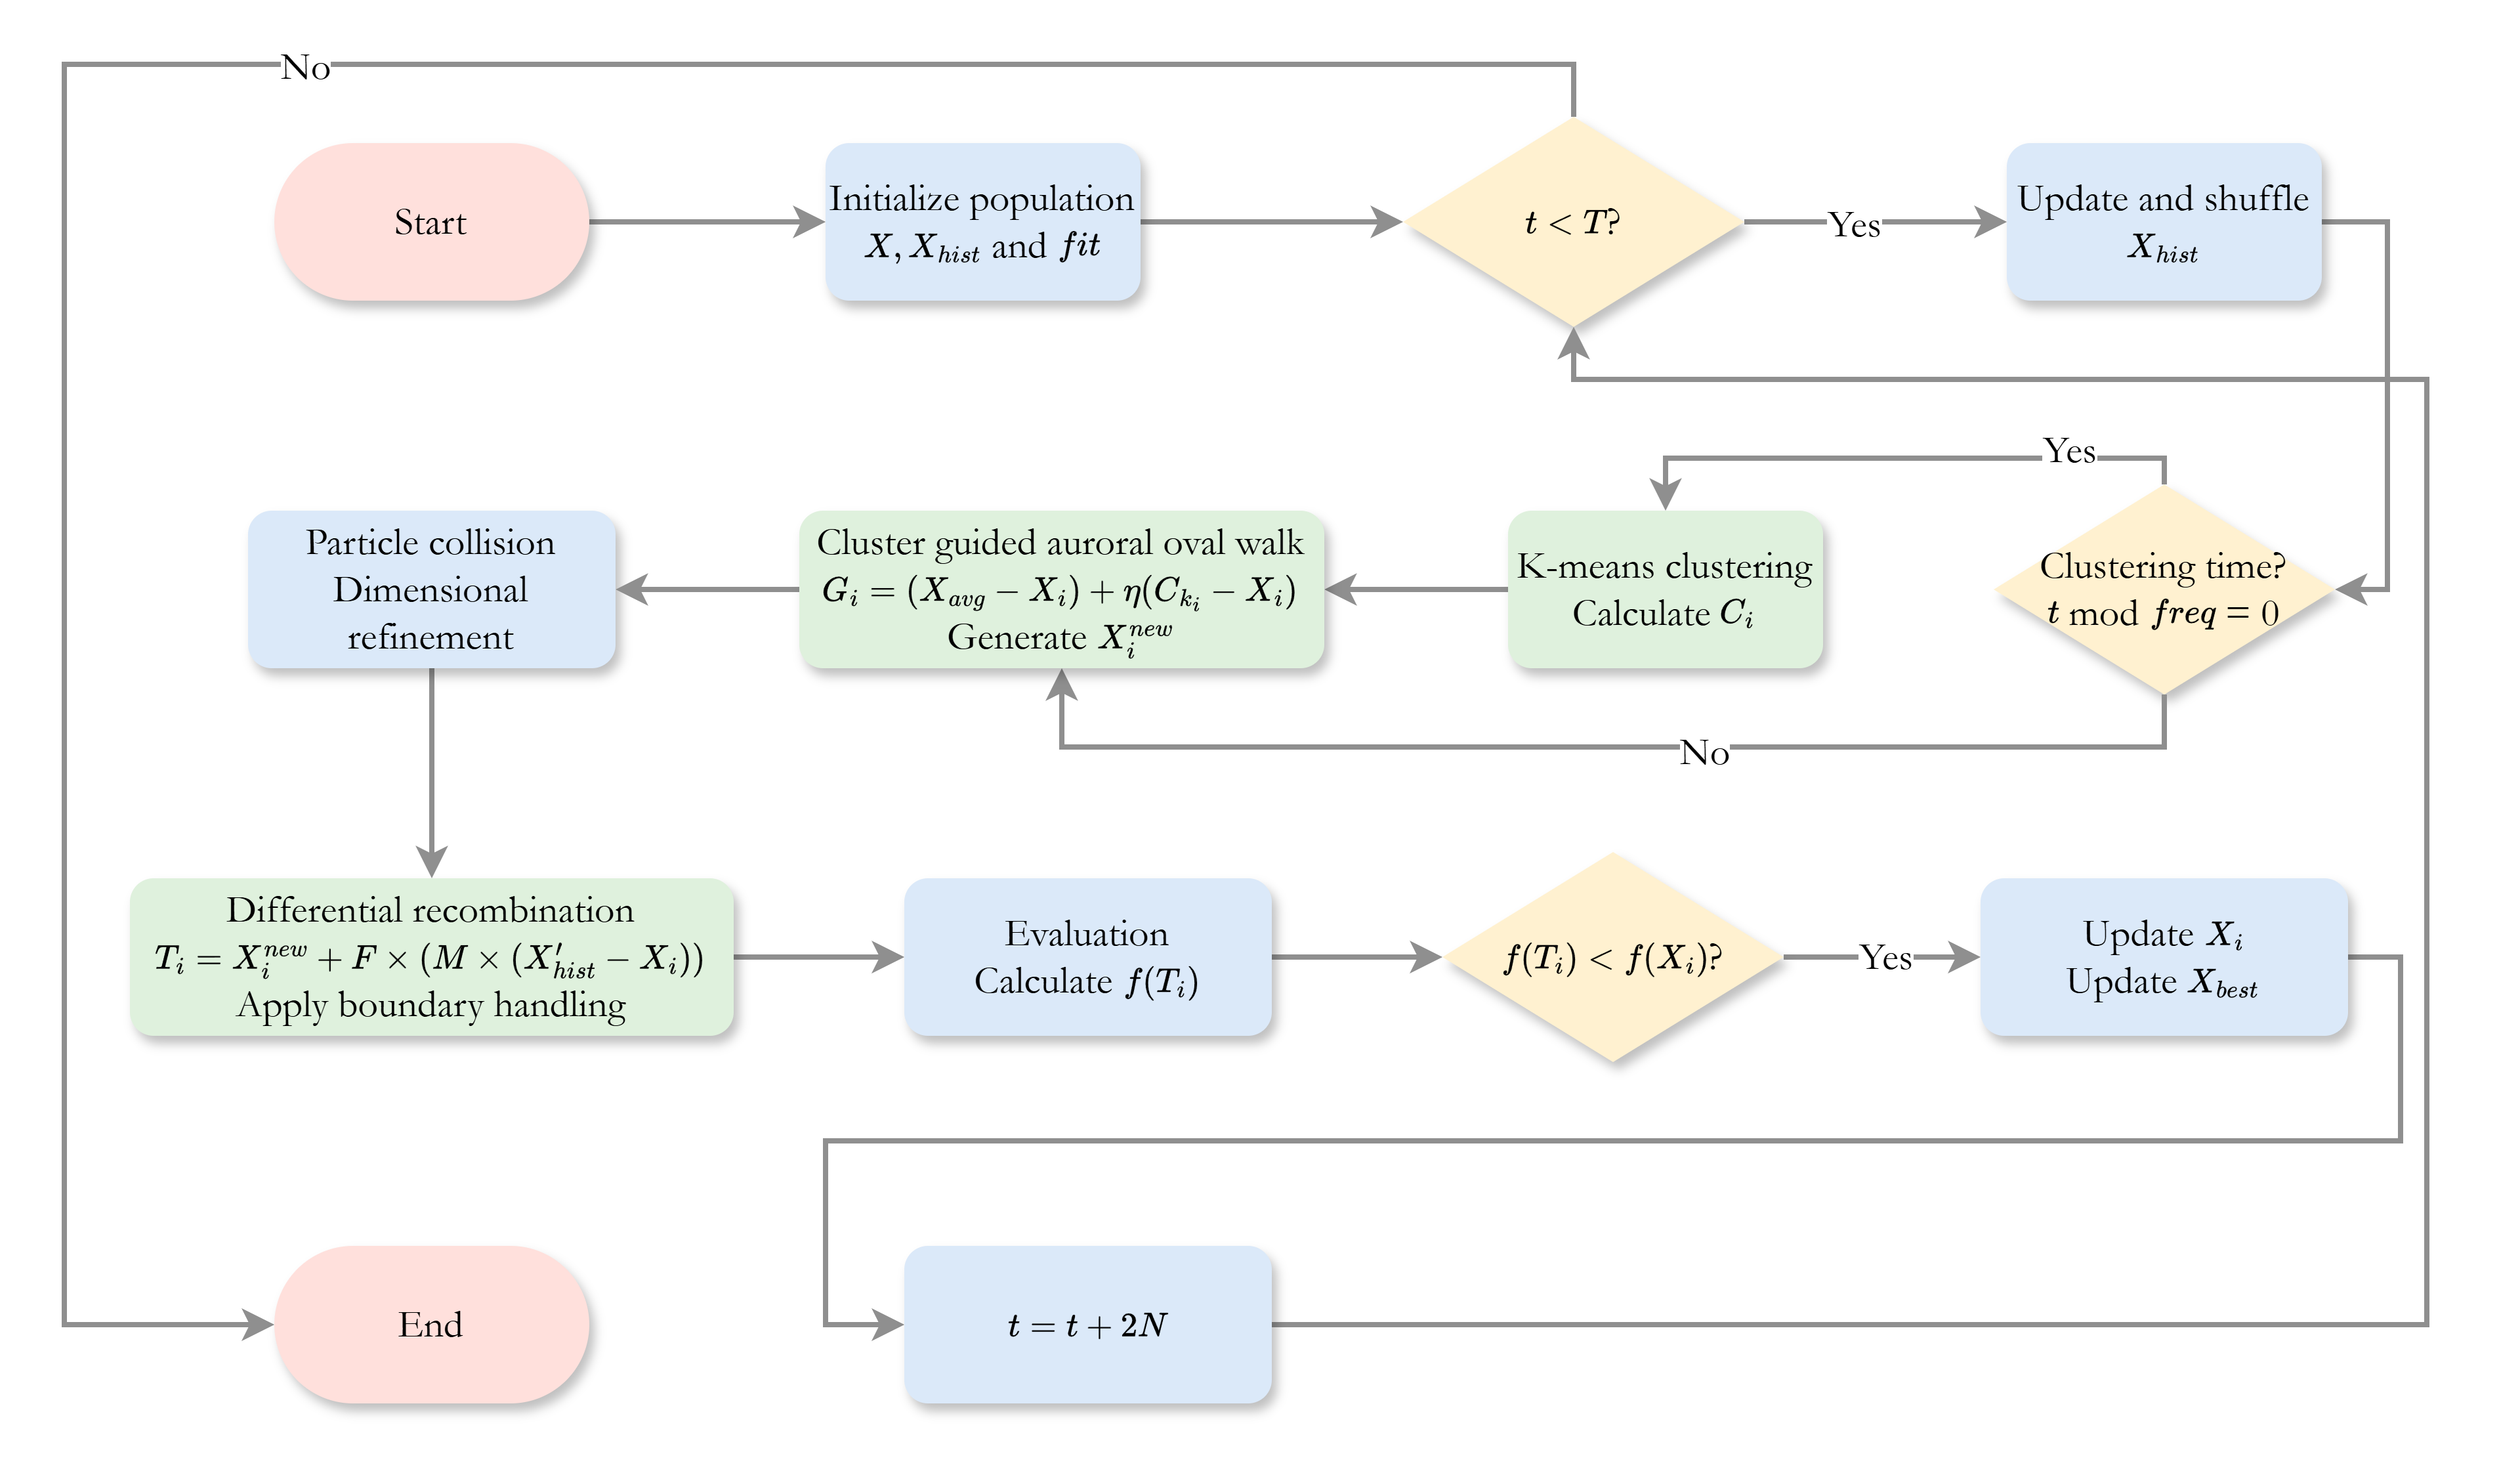
\includegraphics[width=1\textwidth]{CDPLO-flowchart.png}
	\caption{CDPLO flowchart.}
	\label{fig: CDPLO-flowchart}
\end{figure}

\section{Benchmark validation}
% This section detail the benchmark validation
In this section, we conducted three experiment for the comprehensive evaluation of the proposed CDPLO, regarding the exploration and exploitation quality during the evolving process; the contribution of the cluster guidance strategy and differential recombination strategy to the CDPLO's performance; and how CDPLO compared with the state-of-the-art optimizers.

All experiment setup in this study follows a maximum objective function evalutions $T$ of 300,000, population size $pop_size$ of 30, and 30 independent runs for each of the tested function. All the compared algorithm's parameter follows their original published if not specified additionally. And the benchmark test suite is the most popular and well established IEEE CEC 2017. To the best of our knowledge, it is the mostly benchmarked test suite in single objective optimization testing.

\subsection{Quality analysis of CDPLO}
We conducted the balance and diversity analysis to the proposed CDPLO vs. original PLO optimizer to test the changes of the exploration and exploitation rates after the introduction of two strategies. Four functions are selected for the this experiment, single module function F1 is selected to test the exploitation ability of the algorithms, due to the only optimum exist in the fitness landscape. The algorithm have strong exploitation ability will have a larger convergence speed and better solution qaulity to the end of the evolution. Multimodule function F5 utlized to benchmark the exploration ability to the algorithms, with complicated fitness landscape and multi optima, it test the algorithm's global exploration ability and local optimum avoidance ability. Hybrid function F13 and Composition function F29 benchmark the algorithm's balance ability between the exploration and the exploitation, only the algorithm have a decent trade-off between those two phase, can the algorithm find the global optimum during the evolution process.

Five columns of plots can be seen in Fig. \ref{fig: CDPLO-BD}, including the 3D function landscape plotted in Fig. \ref{fig: CDPLO-BD}(a), and exploration and exploitation percentage of the CDPLO and original PLO plotted in Fig. \ref{fig: CDPLO-BD}(b) and Fig. \ref{fig: CDPLO-BD}(c). Assisted with the population diversity and algorithm convergence plotted in Fig. \ref{fig: CDPLO-BD}(d) and Fig. \ref{fig: CDPLO-BD}(e).

From the exploration and exploitation rate of the columns (b) and columns (c), the result indicate that the CDPLO improve the performance of PLO by increasing the exploitation ability within evolving. The root cause of the improving comes from the higher exploration rate in the original PLO algorithm which cause the diversity sparse, and could not converge to a refined local area as faster as it should be, thus consume more function evaluation counts while stagnant without improving. The improved exploitation assisted with faster population diversity dimenish lead to a better solution refinement as can been see in the column (d) and column (e), which leverage the searching ability of the original PLO algorithm.

\begin{figure*}[htbp]
  \centering
  \includegraphics[width=\linewidth]{CDPLO-BD.png}
  \caption{Run-time behaviour of CDPLO
           vs.\ the original PLO.
           (a) landscape of the selected functions;
           (b) exploration/exploitation percentages of CDPLO;
           (c) exploration/exploitation percentages of PLO;
           (d) average distance between individuals (population diversity);
           (e) best-so-far fitness curve.}
  \label{fig: CDPLO-BD}
\end{figure*}

\subsection{Ablation study}
We test the contribution of the proposed two strategy to the original PLO algorithm in this section. two more variants are introduced here, CPLO with only cluster guidance are introduced to PLO, and DPLO with only differential recombination are introduced to the PLO. By benchmark those variants performance to the original PLO algorithm, we can observe the contribution of the strategy made to the CDPLO in total. Table \ref{table: PLO variants} describe those variants in detail.

\begin{table}[]
\centering
\caption{PLO and its variations.}
\label{table: PLO variants}
\begin{tabular}{@{}lcc@{}}
\toprule
      & Cluster guidance & Differential recombination \\ \midrule
CDPLO & 1                & 1                          \\
CPLO  & 0                & 0                          \\
DPLO  & 1                & 0                          \\
PLO   & 0                & 0                          \\ \bottomrule
\end{tabular}
\end{table}

The detailed comparison results of CDPLO are shown in the Table \ref{table: CDPLO-Ablation}, including all 29 function in the IEEE CEC 2017 comparison, and the non-parametric analysis of Wilcoxon signed-rank test (WSRT), average rank value (ARV) and Friedman rank (FR) test shown in the last columns of the comparison result. The average fitness value over 30 independent run are reported as Avg, and those independent runs are utilized to calculate the standard devision (Std) to see the robustness and variablity of the algorithm's performance. For easy of recognition of the best result, we bold the best Avg and Std of each testing function. Also we have visulize some of the comparison result to describe the key observations of this experiment.

The result shows that each component contributes, CPLO and DPLO both outperform the baseline, and their fusion CDPLO yield the fastest convergence curve and the best solution quliaty. We present the best-fitness-so-far convergence curve in Fig. \ref{fig: CDPLO-Ablation-CC}, the presented function are single module function F2, hybrid functions F13, F15, F16, F19, and composition function F20. A closer look at the curves we can find that the CDPLO have a significant performance improve compare with the original PLO while only have marginal performance improvement when compare with the CPLO and DPLO. While when compare with the CPLO and DPLO, it is obvious, those two have different performance in those function. With CPLO have better performance in F15 and F20, while in the F2, F13, F16, and F19, DPLO shows better performance trend. In total, the fusion CDPLO exceed all other PLO variants, which demostrate that those two strategies both contribute to the performance of CDPLO algorithm. 

\begin{figure}
\centering
\caption{Convergence curves of the full CDPLO and its
           two single-component variants on six test
           functions.}
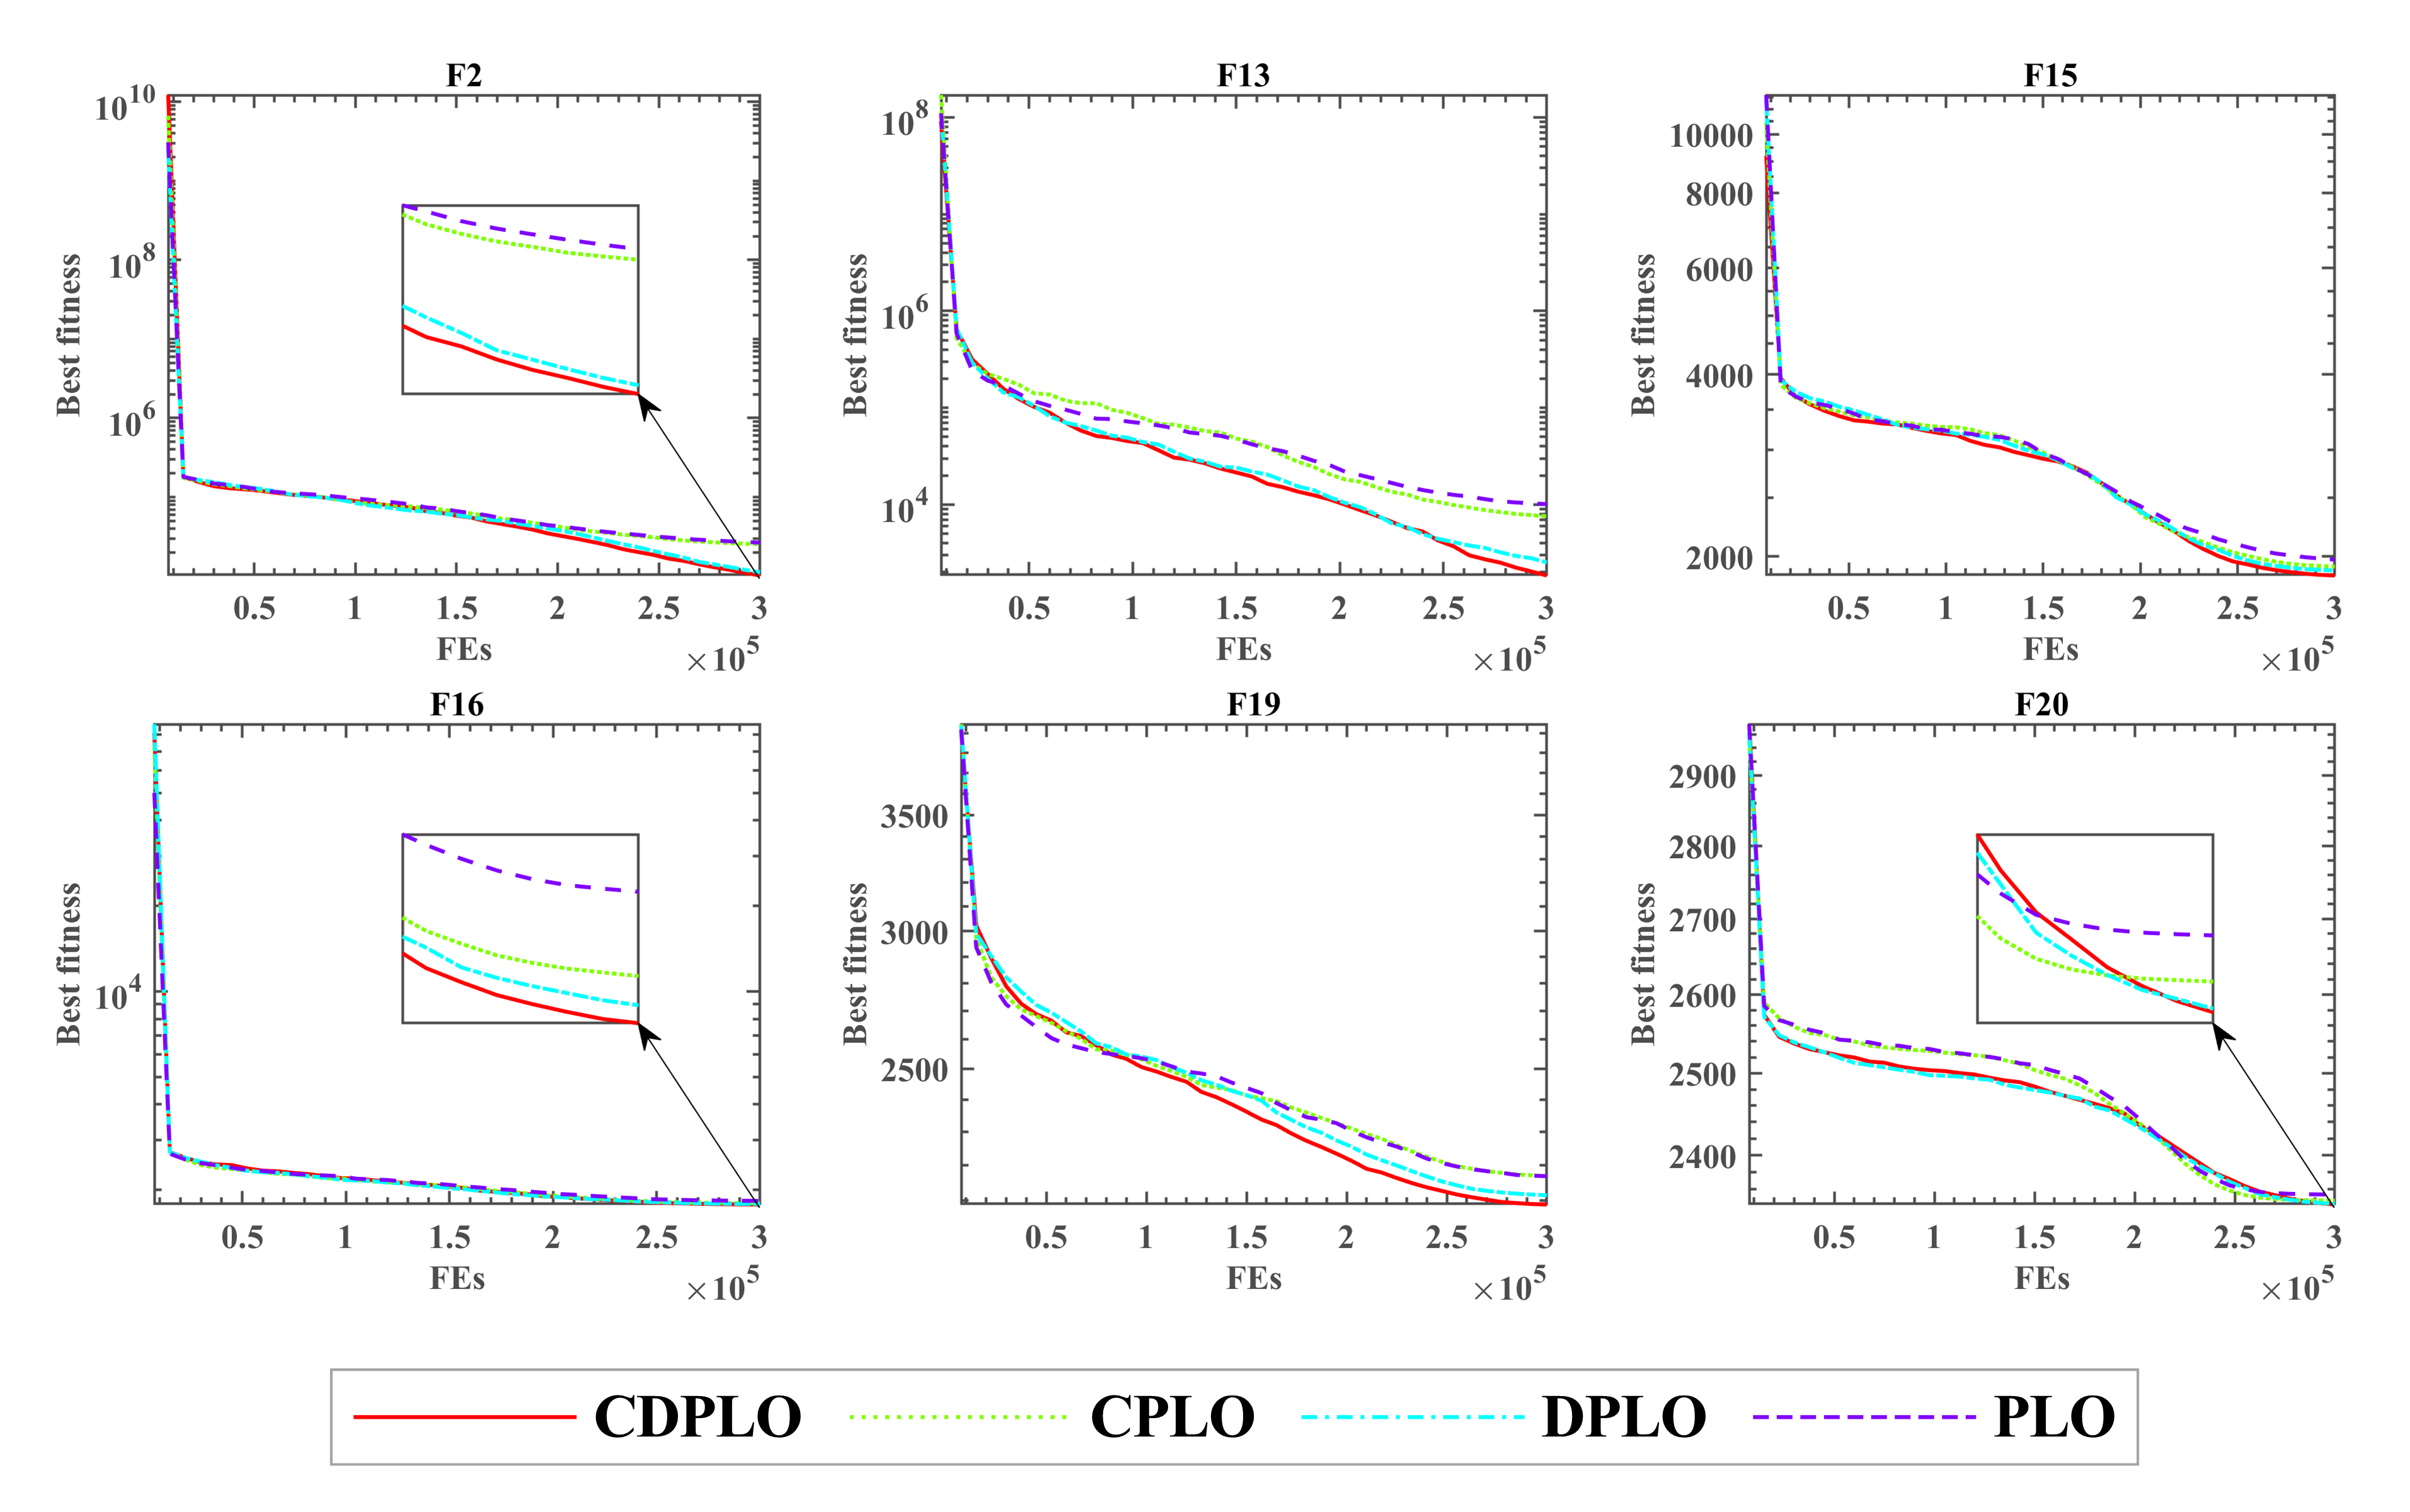
\includegraphics[width=\linewidth]{CDPLO-Ablation}
\label{fig: CDPLO-Ablation-CC}
\end{figure}

For a more comprehensive showing the robustness the algorithm in the test functions, we have visulized the 30 independent runs for those algorithm, since the fitness value may vary in a very long range, we have made the appropriate scale for the fitness value to better differentiate them while present the result in a decent way. The boxplot result are showin in Fig. \ref{fig: CDPLO-Ablation-boxplot}. The scatter dot and the relative fitness value can be seen in the figure, the lower the bar, the dense the scatter dots, the better the algorithm's robustness and performance. Obviously, the PLO shows the highest bar while a relative sparse scatter dots distribution, while the CPLO and DPLO both have a relative lower bar compare with the original PLO, the fusion of them CDPLO obtain the lowest bar height and the most dense scatter dots in total, represent better robustness and performance over other PLO variants and PLO algorithm.

 \begin{figure}
\centering
\caption{Scaled best fitness (box-and-scatter) of the four
           methods over 30 runs on the same six functions.}
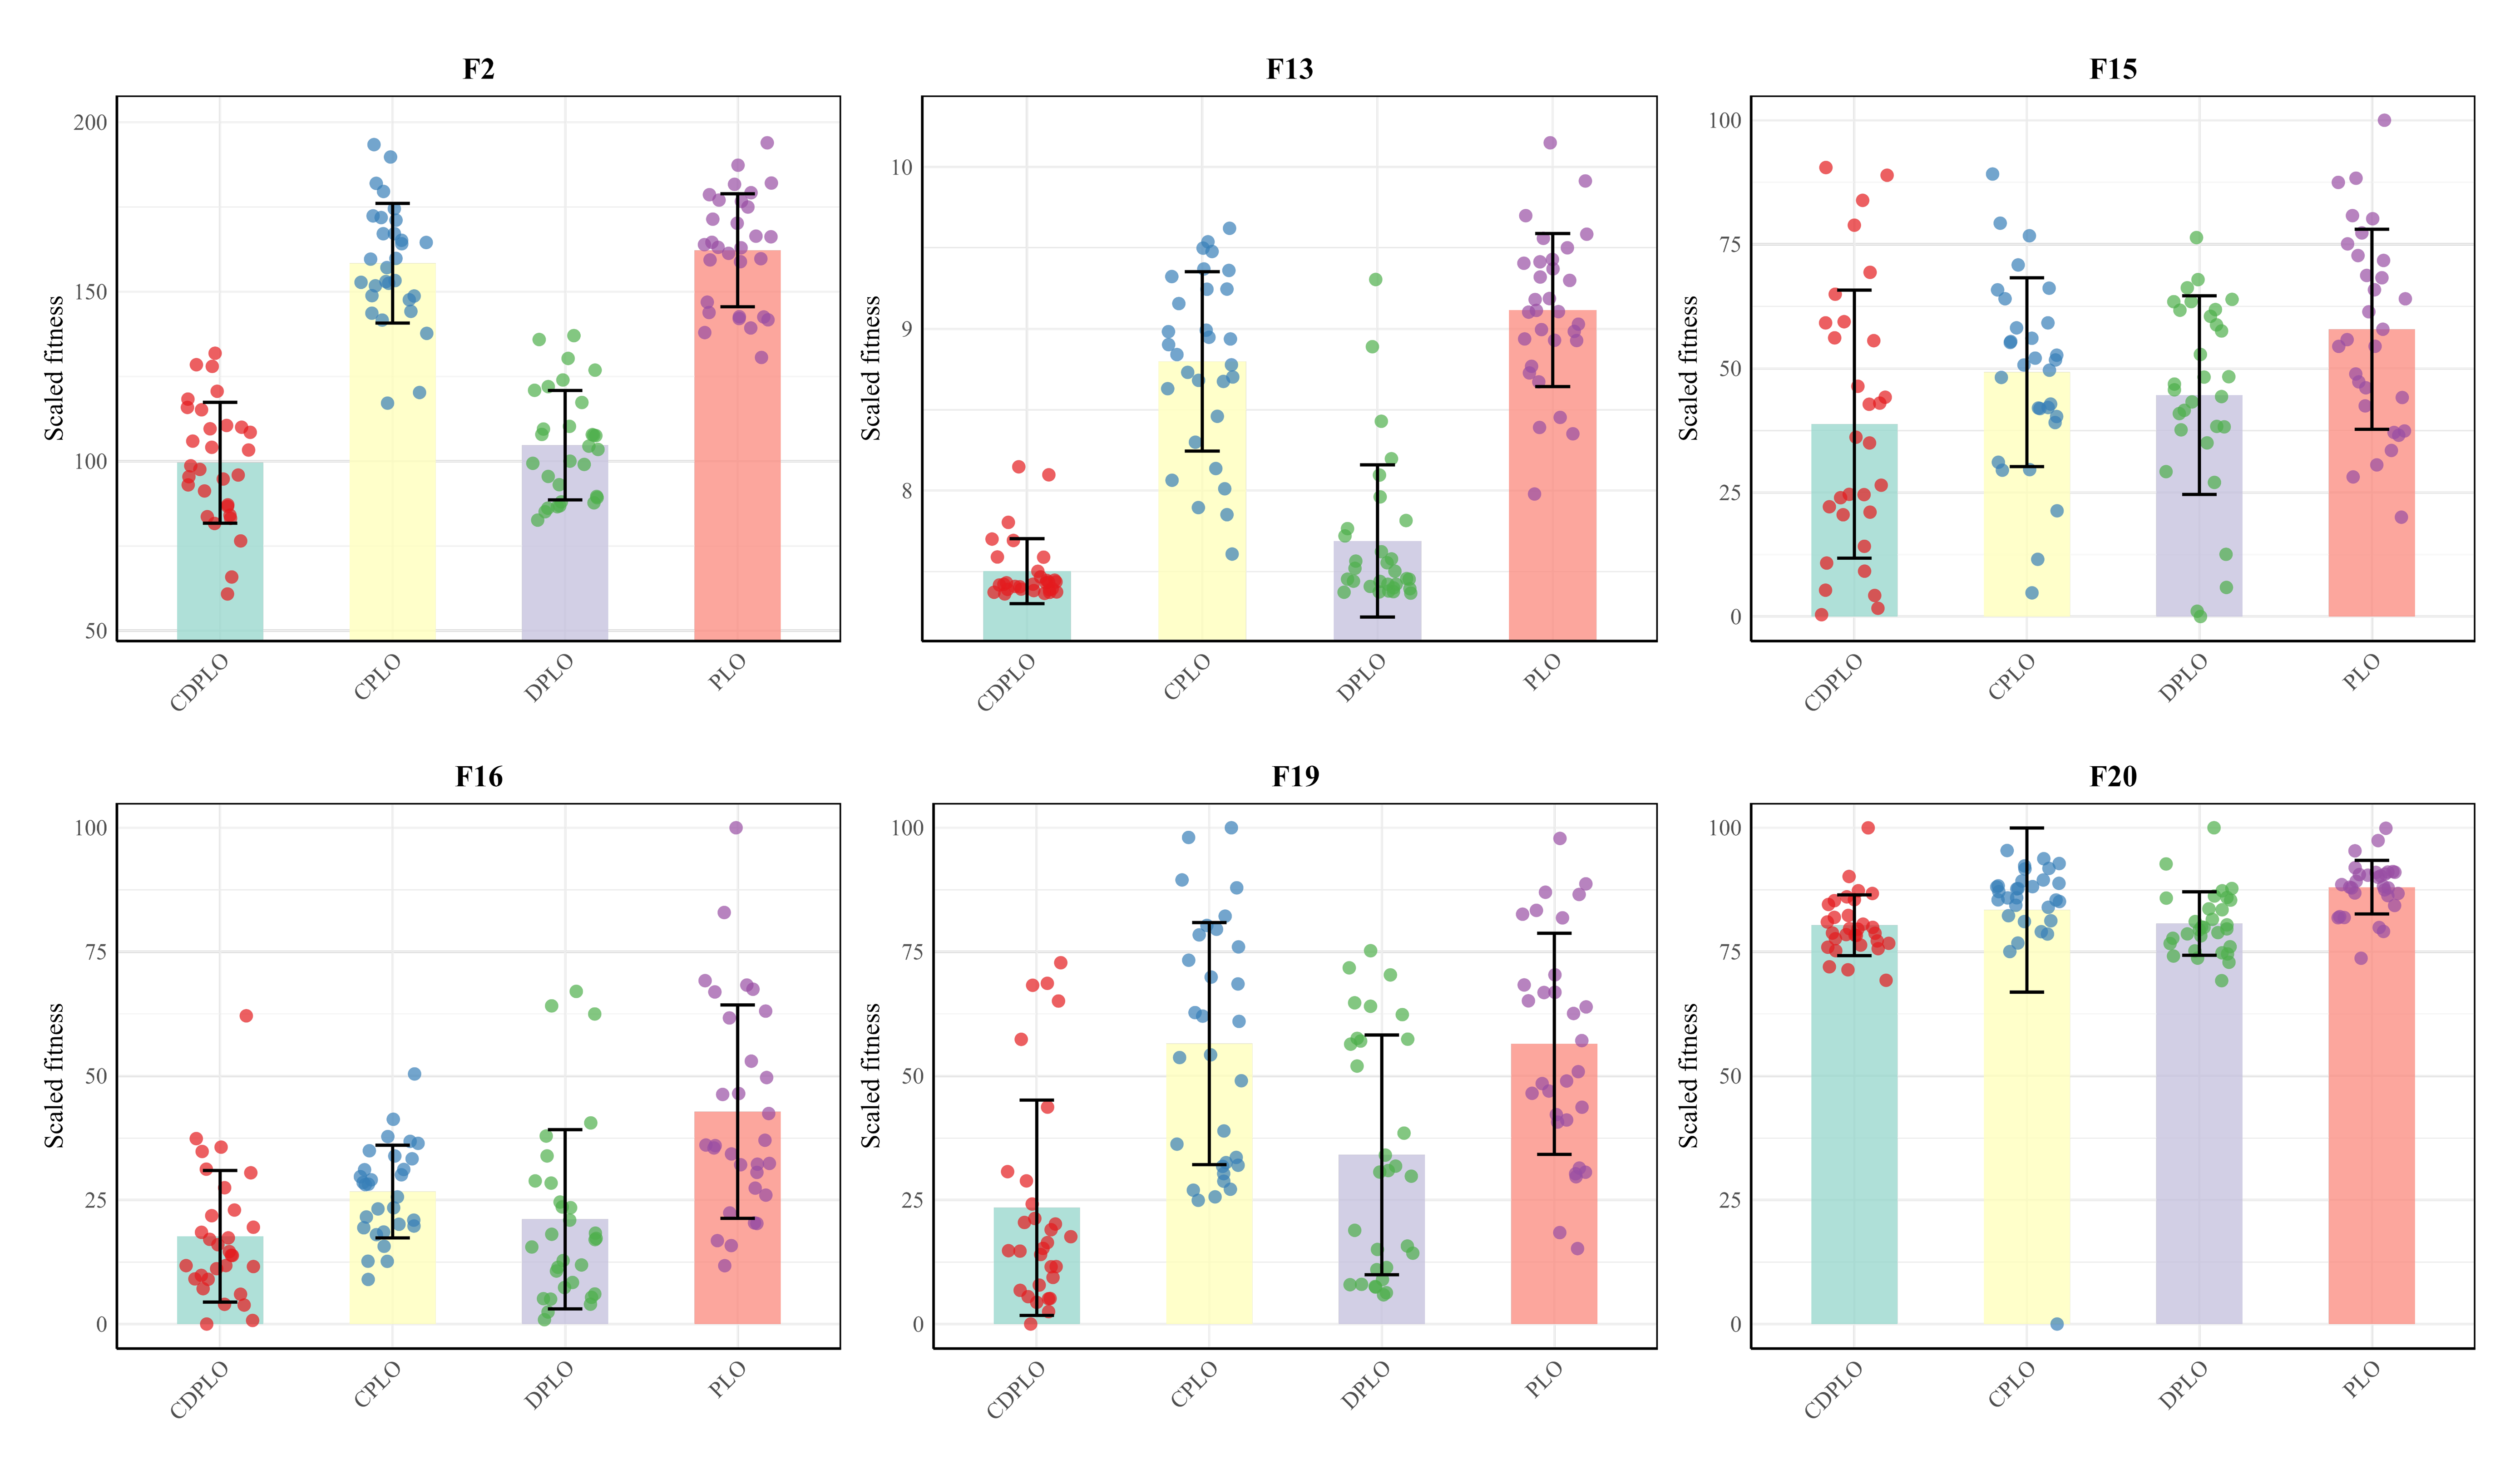
\includegraphics[width=\linewidth]{CDPLO-Ablation-boxplot}
\label{fig: CDPLO-Ablation-boxplot}
\end{figure}

For the sake of better seeing each algorightm performance over each 29 functions, we provide the radar plot in Fig. \ref{fig: Abation-FR}(a), assisted with a ARV and FR value bar plot in Fig. \ref{fig: Ablation-FR}(b).

\begin{figure}
\centering
\caption{Average-rank value (ARV) and Friedman post-hoc ranking
           of the four methods over all 30 CEC 2017 functions.}
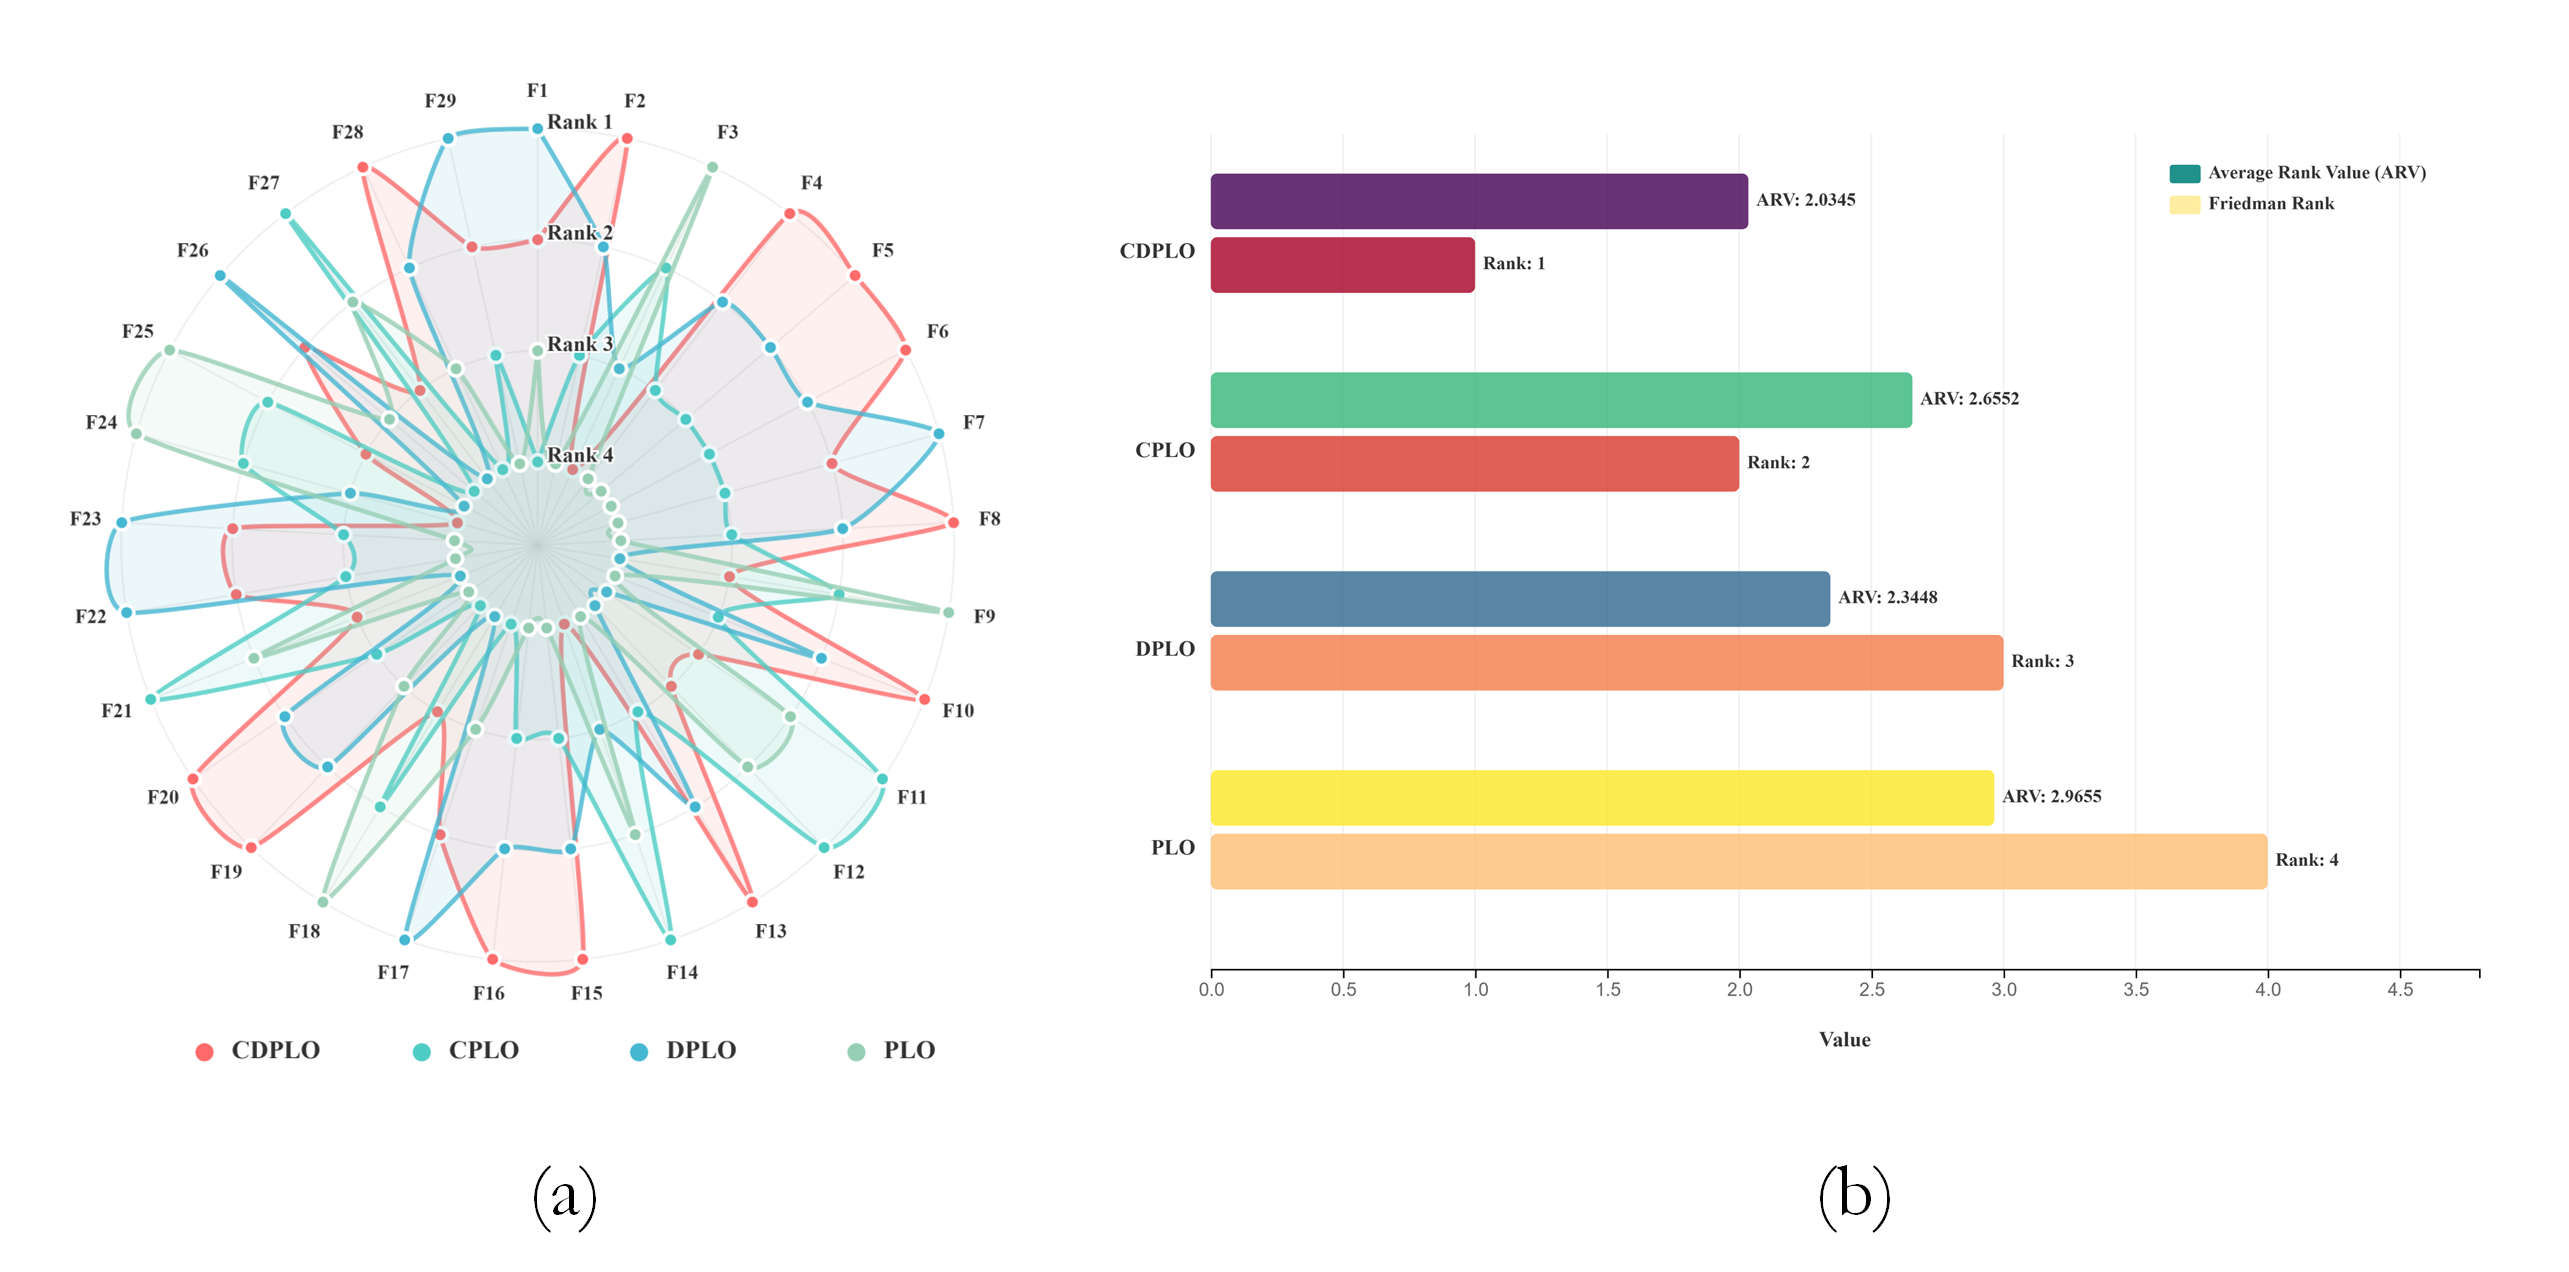
\includegraphics[width=\linewidth]{Ablation-FR}
\label{fig: Ablation-FR}
\end{figure}

\begin{table}
\centering
\caption{Comparison results of PLO and its variants.}
\label{table: CDPLO-Ablation}
\begin{tabular}{@{}lcccccccccccccccc@{}}
\toprule
           & F1                 &                    & F2                 &                    & F3                 &                    & F4                 &                    & F5                 &                    & F6                   &                     & F7                 &                    & F8                 &                    \\ \midrule
Algorithms & Avg                & Std                & Avg                & Std                & Avg                & Std                & Avg                & Std                & Avg                & Std                & Avg                  & Std                 & Avg                & Std                & Avg                & Std                \\
CDPLO      & 5.842E+03          & 3.057E+03          & \textbf{1.022E+04} & 3.529E+03          & 4.948E+02          & 1.071E+01          & \textbf{5.441E+02} & 1.042E+01          & \textbf{6.005E+02} & \textbf{2.867E-01} & \textbf{8.048E+02}   & 1.364E+01           & 8.470E+02          & \textbf{6.478E+00} & \textbf{9.000E+02} & \textbf{4.418E-04} \\
CPLO       & 1.204E+04          & \textbf{2.374E+03} & 2.539E+04          & 5.531E+03          & 4.817E+02          & \textbf{8.858E+00} & 5.469E+02          & \textbf{7.580E+00} & 6.106E+02          & 2.153E+00          & 8.159E+02            & 1.591E+01           & 8.595E+02          & 8.397E+00          & 1.161E+03          & 9.314E+01          \\
DPLO       & \textbf{4.891E+03} & 2.924E+03          & 1.122E+04          & \textbf{3.506E+03} & 4.932E+02          & 9.055E+00          & 5.442E+02          & 9.469E+00          & 6.006E+02          & 3.426E-01          & 8.050E+02            & \textbf{1.033E+01}  & \textbf{8.447E+02} & 6.670E+00          & 9.000E+02          & 5.861E-04          \\
PLO        & 1.152E+04          & 2.482E+03          & 2.659E+04          & 5.377E+03          & \textbf{4.745E+02} & 1.412E+01          & 5.509E+02          & 7.811E+00          & 6.119E+02          & 2.170E+00          & 8.208E+02            & 1.762E+01           & 8.618E+02          & 1.353E+01          & 1.219E+03          & 1.261E+02          \\
           & F9                 &                    & F10                &                    & F11                &                    & F12                &                    & F13                &                    & F14                  &                     & F15                &                    & F16                &                    \\
Algorithms & Avg                & Std                & Avg                & Std                & Avg                & Std                & Avg                & Std                & Avg                & Std                & Avg                  & Std                 & Avg                & Std                & Avg                & Std                \\
CDPLO      & 4.125E+03          & \textbf{2.812E+02} & \textbf{1.145E+03} & 2.036E+01          & 5.615E+05          & 3.423E+05          & 1.753E+04          & 1.504E+04          & \textbf{1.852E+03} & \textbf{4.633E+02} & 4.904E+03            & 5.440E+03           & \textbf{1.859E+03} & 1.642E+02          & \textbf{1.775E+03} & 2.867E+01          \\
CPLO       & 3.304E+03          & 3.061E+02          & 1.158E+03          & \textbf{1.282E+01} & \textbf{4.193E+05} & 3.288E+05          & \textbf{1.364E+04} & 6.008E+03          & 7.576E+03          & 3.712E+03          & \textbf{3.811E+03}   & \textbf{7.657E+02}  & 1.923E+03          & \textbf{1.156E+02} & 1.795E+03          & \textbf{2.019E+01} \\
DPLO       & 4.198E+03          & 2.977E+02          & 1.148E+03          & 2.439E+01          & 6.724E+05          & 4.806E+05          & 2.063E+04          & 1.479E+04          & 2.531E+03          & 1.983E+03          & 4.807E+03            & 4.754E+03           & 1.895E+03          & 1.217E+02          & 1.783E+03          & 3.904E+01          \\
PLO        & \textbf{3.277E+03} & 3.238E+02          & 1.158E+03          & 1.628E+01          & 4.269E+05          & \textbf{2.217E+05} & 1.468E+04          & \textbf{3.776E+03} & 1.011E+04          & 4.829E+03          & 4.684E+03            & 1.397E+03           & 1.975E+03          & 1.225E+02          & 1.829E+03          & 4.650E+01          \\
           & F17                &                    & F18                &                    & F19                &                    & F20                &                    & F21                &                    & F22                  &                     & F23                &                    & F24                &                    \\
Algorithms & Avg                & Std                & Avg                & Std                & Avg                & Std                & Avg                & Std                & Avg                & Std                & Avg                  & Std                 & Avg                & Std                & Avg                & Std                \\
CDPLO      & 5.787E+04          & 3.512E+04          & 5.940E+03          & 5.884E+03          & \textbf{2.088E+03} & \textbf{5.257E+01} & \textbf{2.342E+03} & 9.317E+00          & 3.076E+03          & 1.434E+03          & 2.693E+03            & 1.146E+01           & 2.861E+03          & 7.326E+00          & 2.887E+03          & 4.184E-01          \\
CPLO       & 1.208E+05          & 6.141E+04          & 3.179E+03          & \textbf{7.899E+02} & 2.169E+03          & 5.910E+01          & 2.346E+03          & 2.516E+01          & \textbf{2.311E+03} & \textbf{4.373E+00} & 2.698E+03            & 7.392E+00           & 2.866E+03          & \textbf{6.529E+00} & 2.885E+03          & 1.415E+00          \\
DPLO       & \textbf{5.449E+04} & \textbf{3.183E+04} & 6.544E+03          & 6.183E+03          & 2.114E+03          & 5.853E+01          & 2.342E+03          & 9.737E+00          & 3.461E+03          & 1.572E+03          & \textbf{2.692E+03}   & 8.987E+00           & \textbf{2.859E+03} & 9.045E+00          & 2.887E+03          & \textbf{3.400E-01} \\
PLO        & 1.169E+05          & 4.591E+04          & \textbf{3.110E+03} & 8.667E+02          & 2.168E+03          & 5.400E+01          & 2.353E+03          & \textbf{8.224E+00} & 2.641E+03          & 8.616E+02          & 2.701E+03            & \textbf{6.094E+00}  & 2.869E+03          & 8.906E+00          & \textbf{2.885E+03} & 1.577E+00          \\
           & F25                &                    & F26                &                    & F27                &                    & F28                &                    & F29                &                    & \multicolumn{2}{c}{Statistical comparison} &                    &                    &                    &                    \\
Algorithms & Avg                & Std                & Avg                & Std                & Avg                & Std                & Avg                & Std                & Avg                & Std                & WSRT                 & FR                  &                    &                    &                    &                    \\
CDPLO      & 3.968E+03          & \textbf{1.126E+02} & 3.202E+03          & 5.059E+00          & 3.218E+03          & 1.478E+01          & \textbf{3.406E+03} & 3.801E+01          & 1.148E+04          & \textbf{2.484E+03} & \textbf{2.0345}      & \textbf{1}          &                    &                    &                    &                    \\
CPLO       & 3.950E+03          & 4.269E+02          & 3.203E+03          & \textbf{3.668E+00} & \textbf{3.214E+03} & \textbf{4.843E+00} & 3.466E+03          & 5.797E+01          & 1.885E+04          & 5.045E+03          & 2.6552               & 3                   &                    &                    &                    &                    \\
DPLO       & 3.997E+03          & 1.297E+02          & \textbf{3.202E+03} & 4.429E+00          & 3.222E+03          & 1.997E+01          & 3.406E+03          & \textbf{3.078E+01} & \textbf{1.036E+04} & 4.291E+03          & 2.3448               & 2                   &                    &                    &                    &                    \\
PLO        & \textbf{3.811E+03} & 5.609E+02          & 3.202E+03          & 4.154E+00          & 3.214E+03          & 5.381E+00          & 3.441E+03          & 4.995E+01          & 2.039E+04          & 5.225E+03          & 2.9655               & 4                   &                    &                    &                    &                   \\ \bottomrule
\end{tabular}
\end{table}

\subsection{Testing on IEEE CEC 2017}
% This section should show the statistic result and the convergence curve (compare with 9 optimizer)
To comprehensive benchmark the performance of the proposed CDPLO performance, we compare it with 9 state-of-the-art optimization method proposed recently. Black-winged Kite Algorithm (BKA) \ref{}, Status-Based Optimization (SBO) \ref{}, IVY algorithm (IVY) \ref{}, Cross Aaptive Grey Wolf Optimization (CAGWO) \ref{}, Roulette wheel and Mutation improved RIME (RMRIME) \ref{}, Slime Mould Algorithm incorporating Differential Evolution and Powell mechanism (PSMADE) \ref{}, Double adaptive Random spare reinforced Whale Optimization Algorithm (RDWOA) \ref{}, Elite Opposition-Based Learning mutation enhanced Sparrow Search Algorithm (EOBLSSA) \ref{}, Generalized Oppositional Teaching Learning Based Optimization (GOTLBO) \ref{}. We present the comparison results in Table \ref{table: CDPLO-Cmp}, with the best results bolded for better recognization. Also, the non-parametric statistic analysis are included in the last three columns of the table, including the WSRT result, the ARV result and the FR result. The result indicate the proposed CDPLO have a comparative performance among all the peers compared.

We select six functions to visualize the comparison result, the convergence curves are presented in the Fig. \ref{fig: CDPLO-Cmp}, the selected functions are multimodal functions F5 and F8, hybrid functions F15 and F19, composite functions F23 and F25. Due to the inherent overly diversity population of the PLO algorithm, the proposed CDPLO algorithm did not show the fastest convergence curves in the plots, while the introduction of the cluster guidance and the differential recombination, the escape local optima ability of CDPLO and the solution quality had been greatly refined. So although the convergence curves is not so fast in showing in the plot, the solution quality is indeed very comparitive compare with the peers.

\begin{figure}
\caption{Convergence behaviour of CDPLO versus nine
           competitors on six representative CEC 2017 functions.}
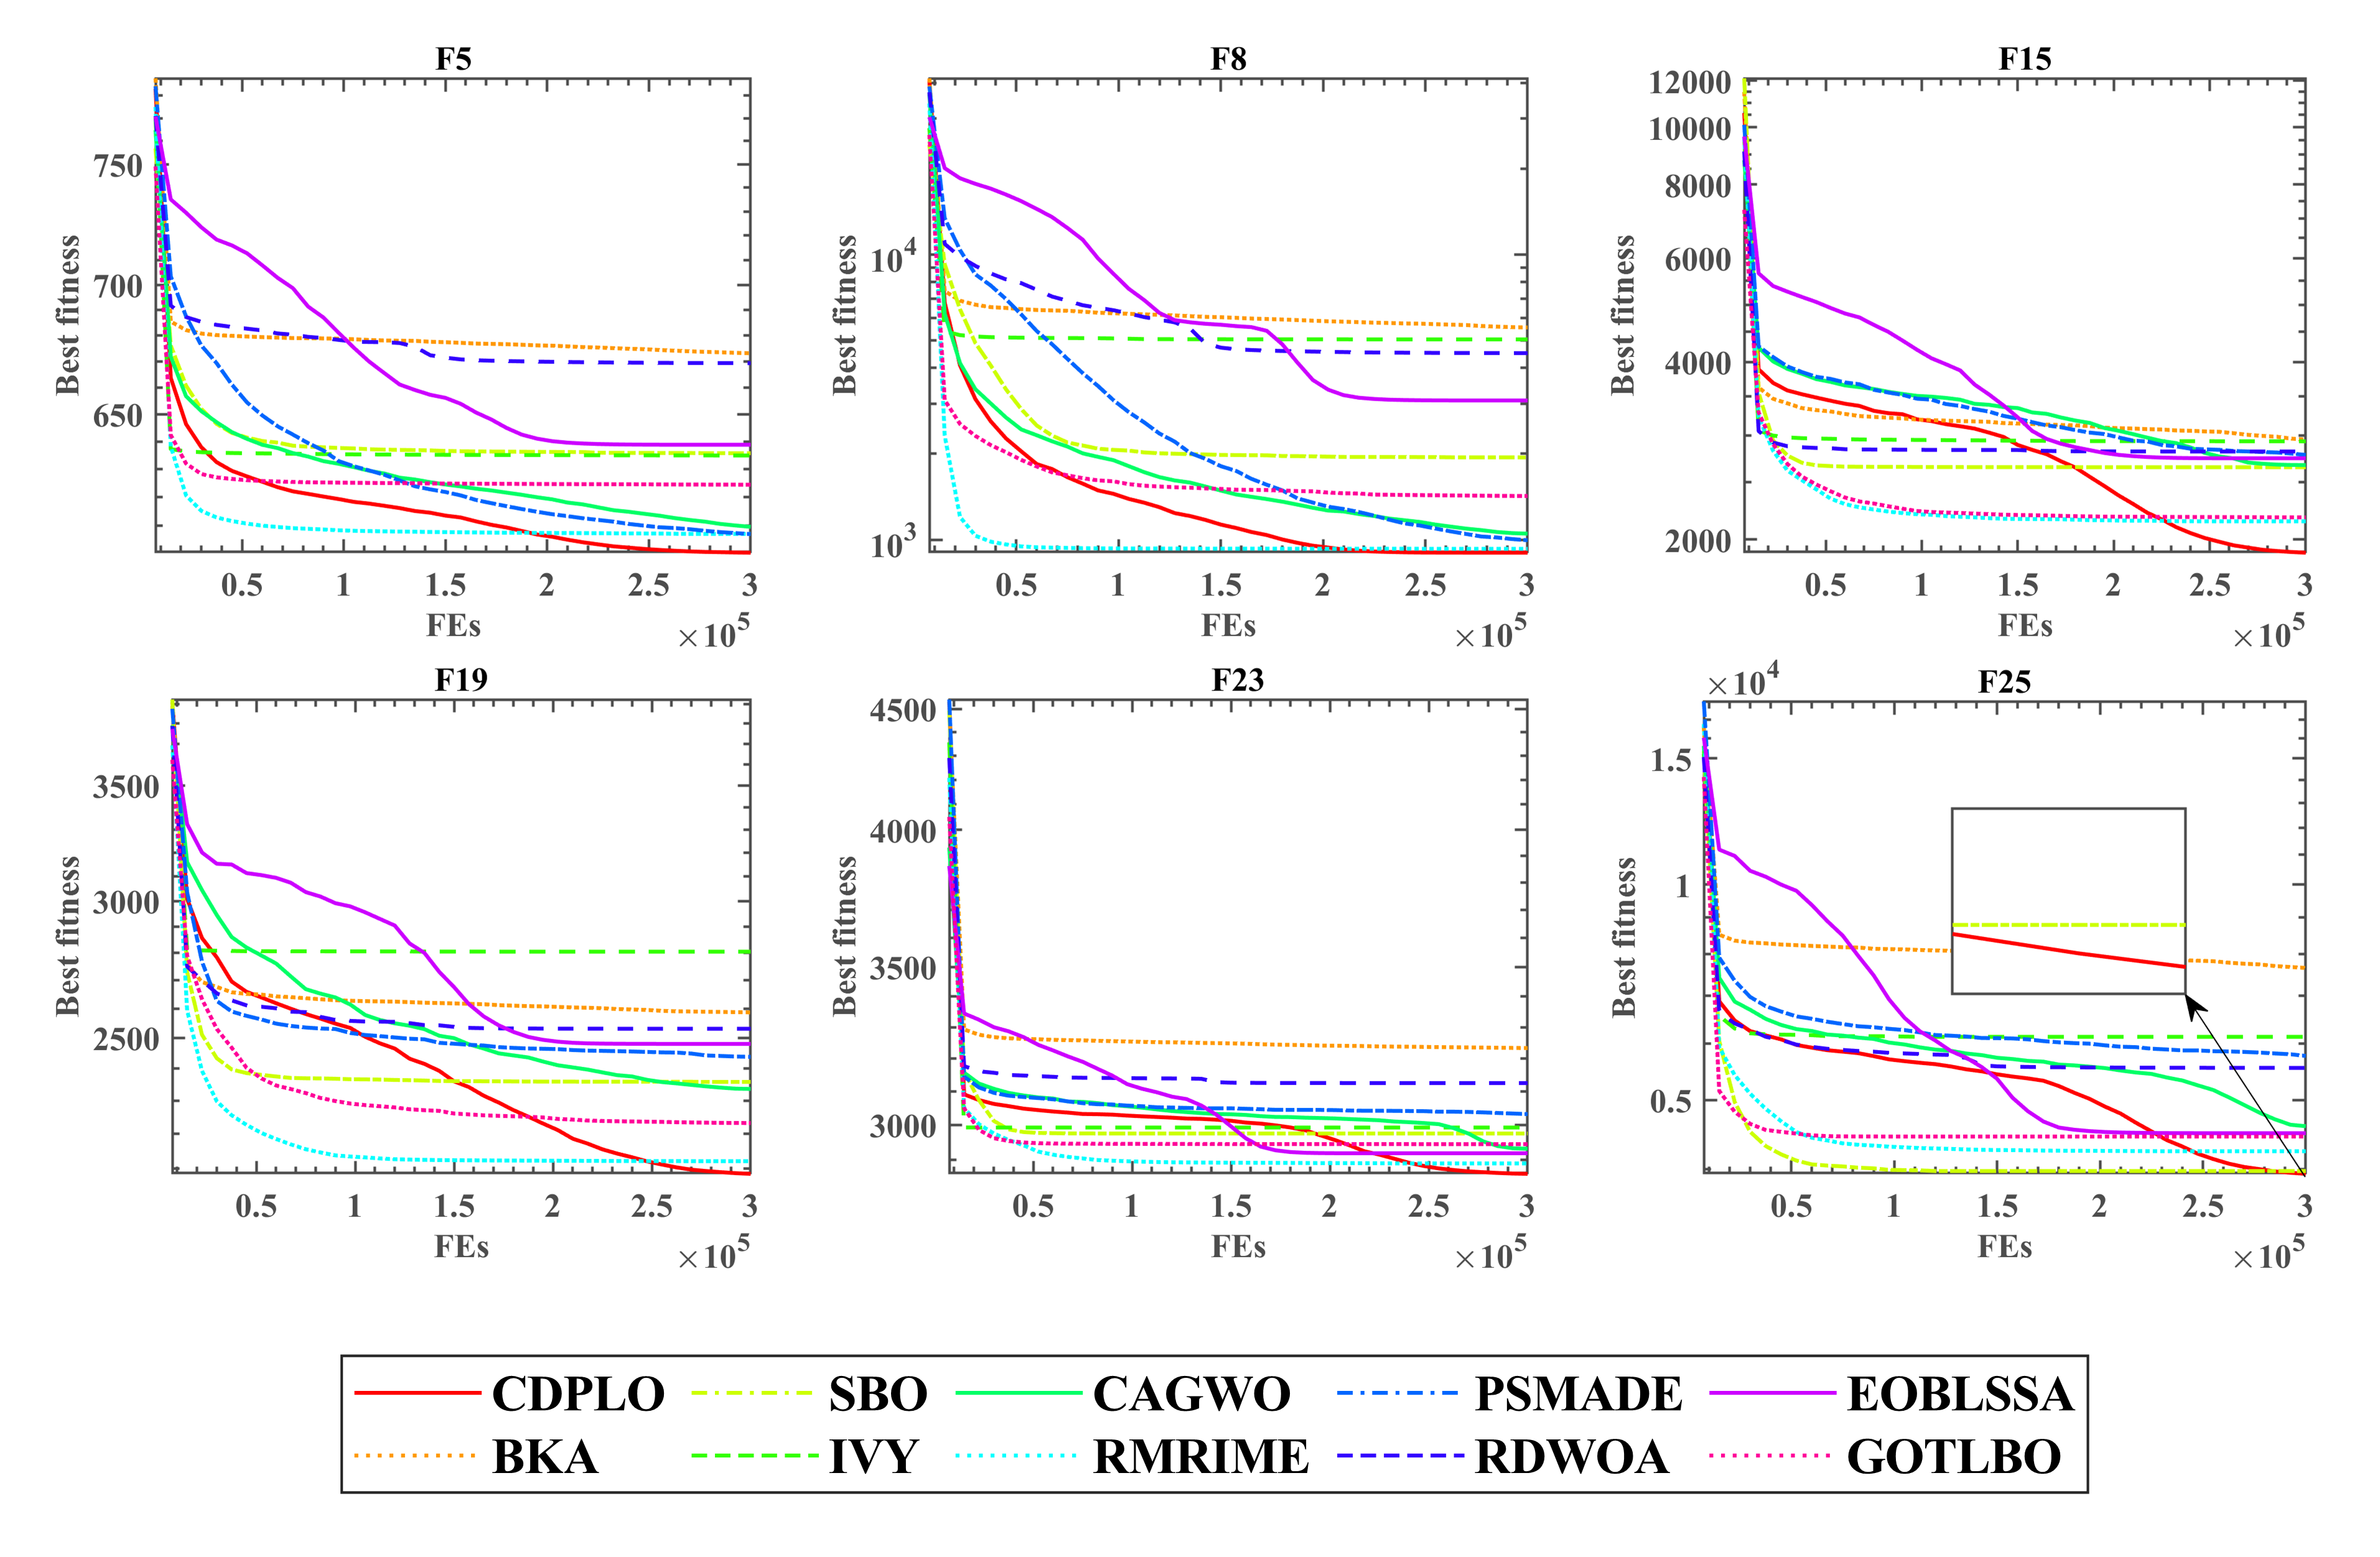
\includegraphics[width=\linewidth]{CDPLO-Cmp}
\label{fig: CDPLO-Cmp}
\end{figure}

Besides, we provide the scatter dots of 30 independent runs of those algorithm and their relative average fitness on selected functions to differentiate their variability during optimization. The plots are presented in the Fig. \ref{CDPLO-Cmp-boxplot}, we can seen that the proposed CDPLO obtain the densest dots in the plots, and the lowest fitness value compare with the peers. This shows the strong robustness of the proposed CDPLO algorithm and its performance. Also, we visulize those algorithm in each of the CEC 2017 functions rank in a radar plot in Fig. \ref{Cmp-FR}(a), and the FR result and AVR result in Fig. \ref{Cmp-FR}(b). Seen from those two figures, the CDPLO have otained the most first rank in the radar plot while shows the lowest FR value and ARV value in the bar plot. Those results strongly indicate the proposed CDPLO have relative superior performance to the peers. For further showing the CDPLO's ability in real-world application, we conducted a feature selection task for preeclampsia prediction.

\begin{figure}
\caption{Scaled best fitness (box-and-scatter) for the ten
           algorithms.}
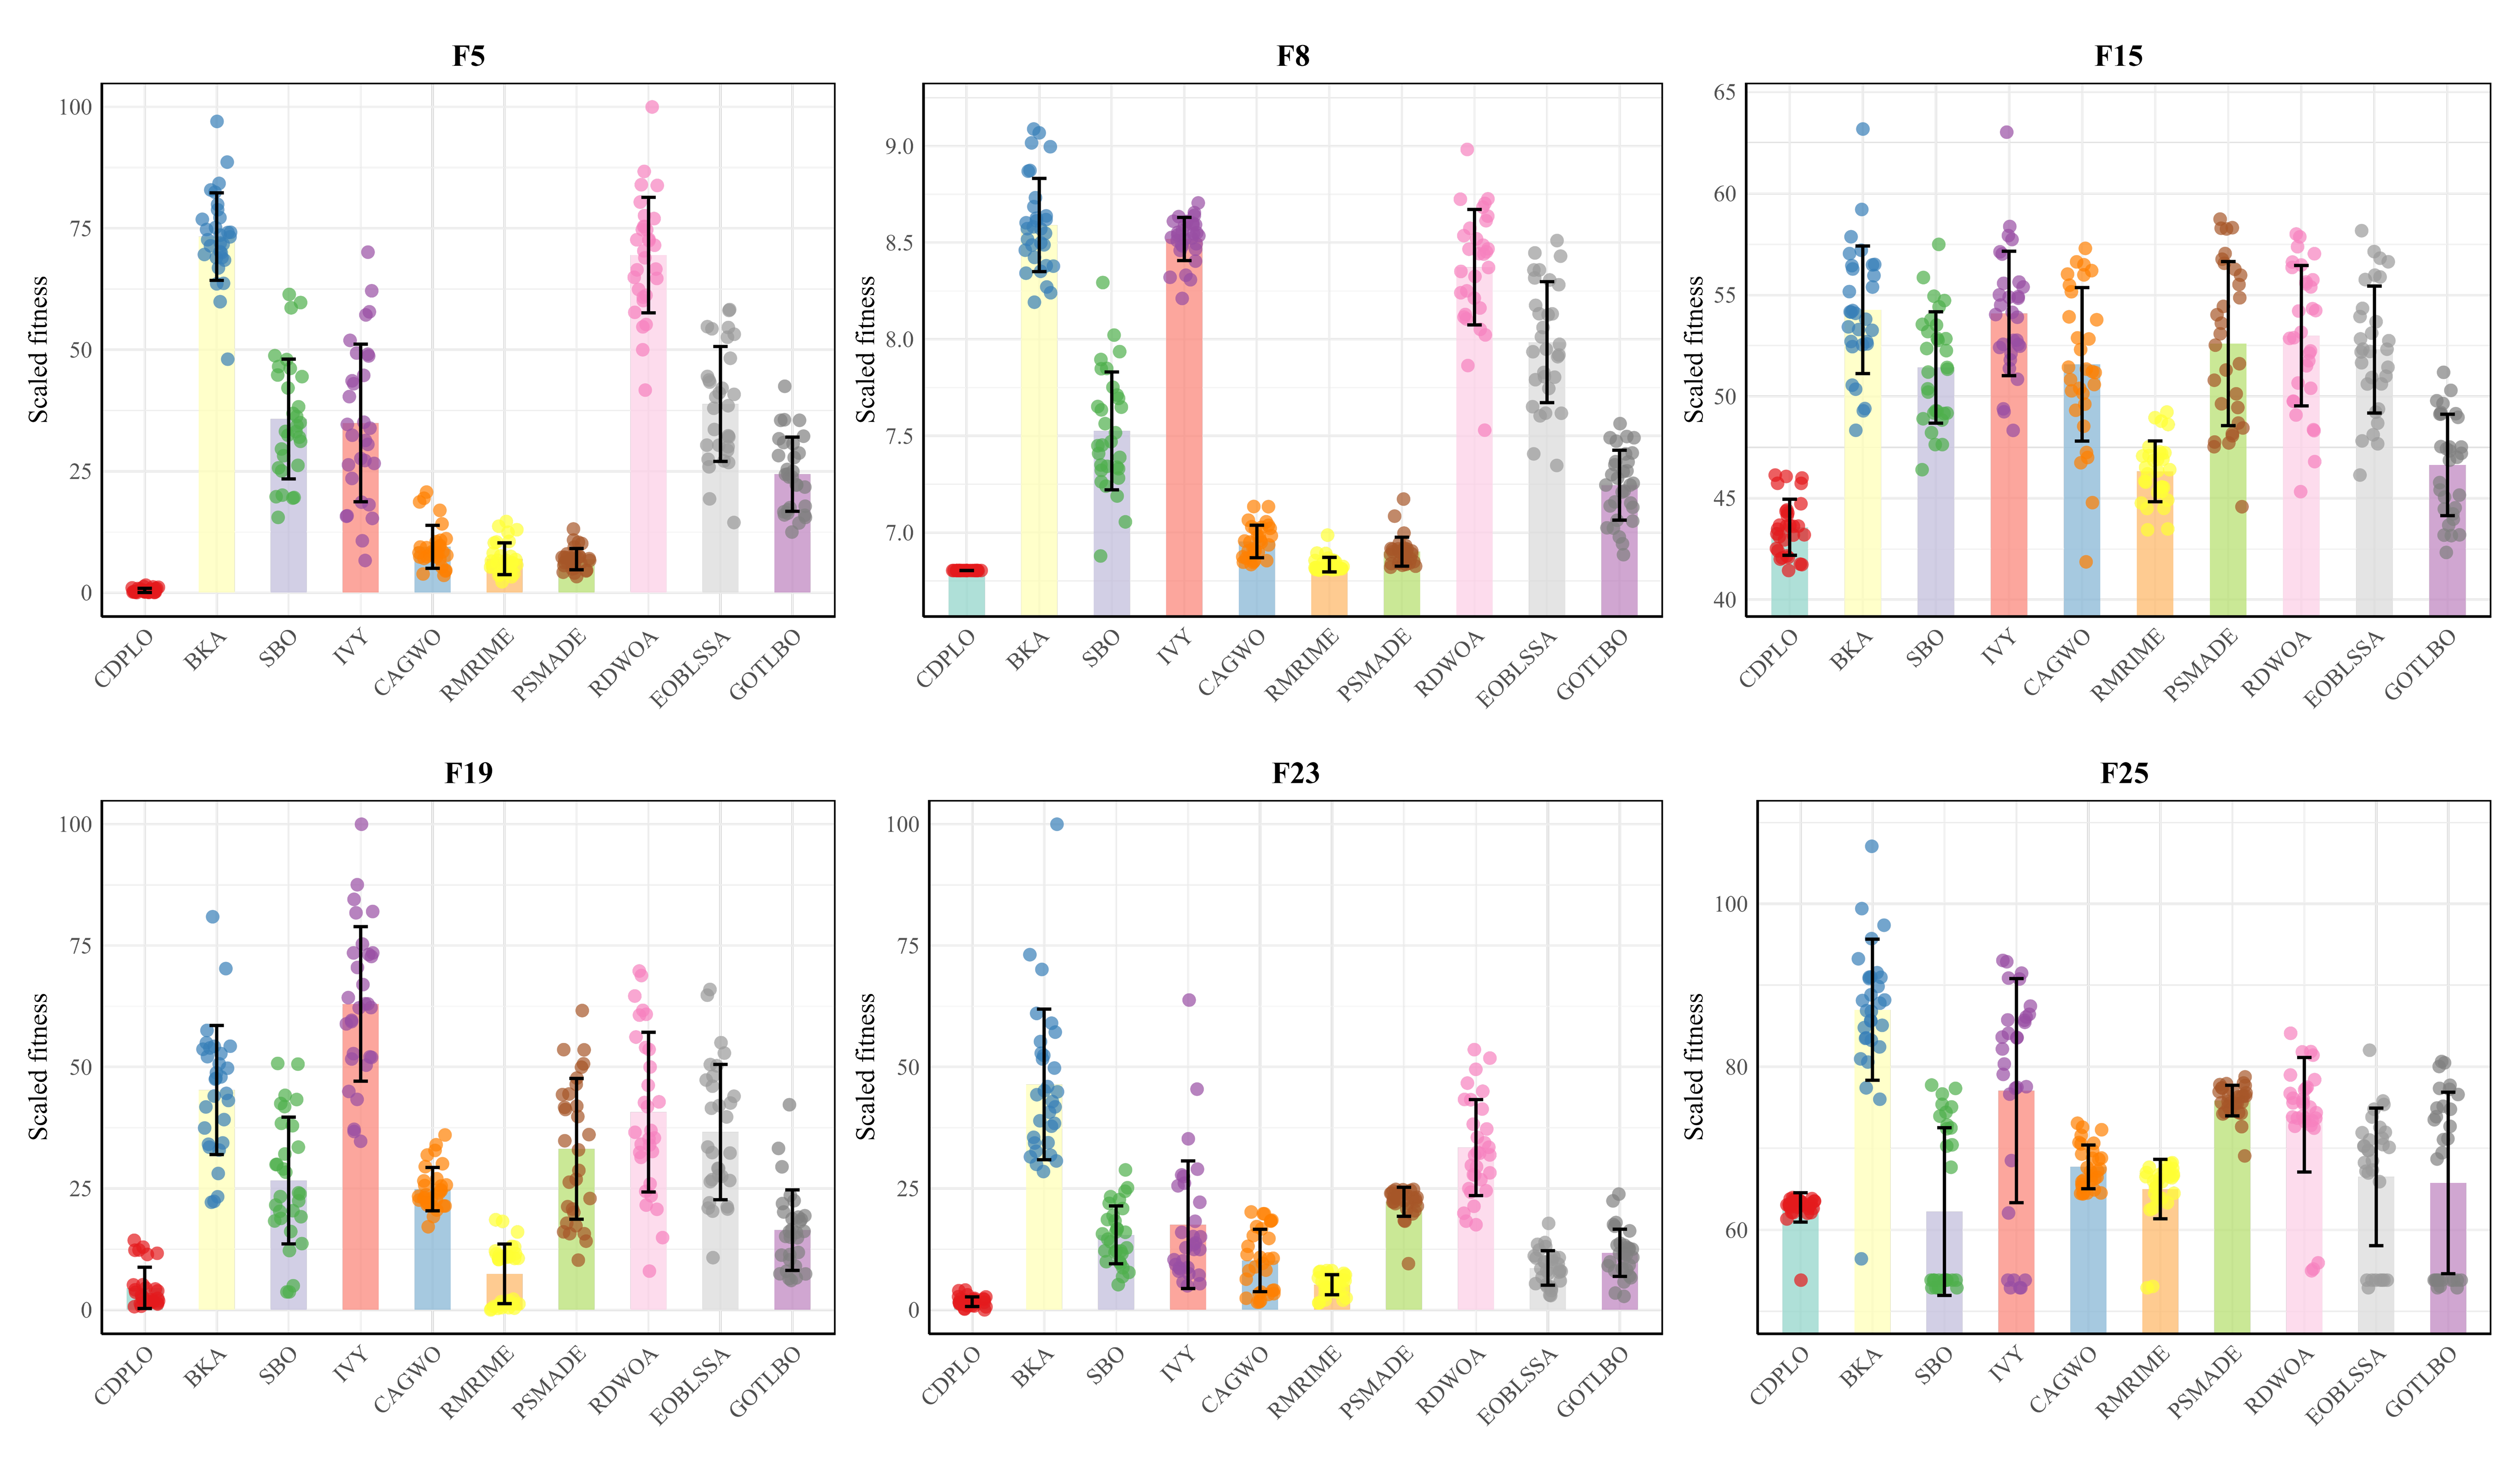
\includegraphics[width=\linewidth]{CDPLO-Cmp-boxplot}
\label{fig: CDPLO-Cmp-boxplot}
\end{figure}

\begin{figure}
\caption{Global ranking on the full 30-function suite:
           average-rank value and Friedman test.}
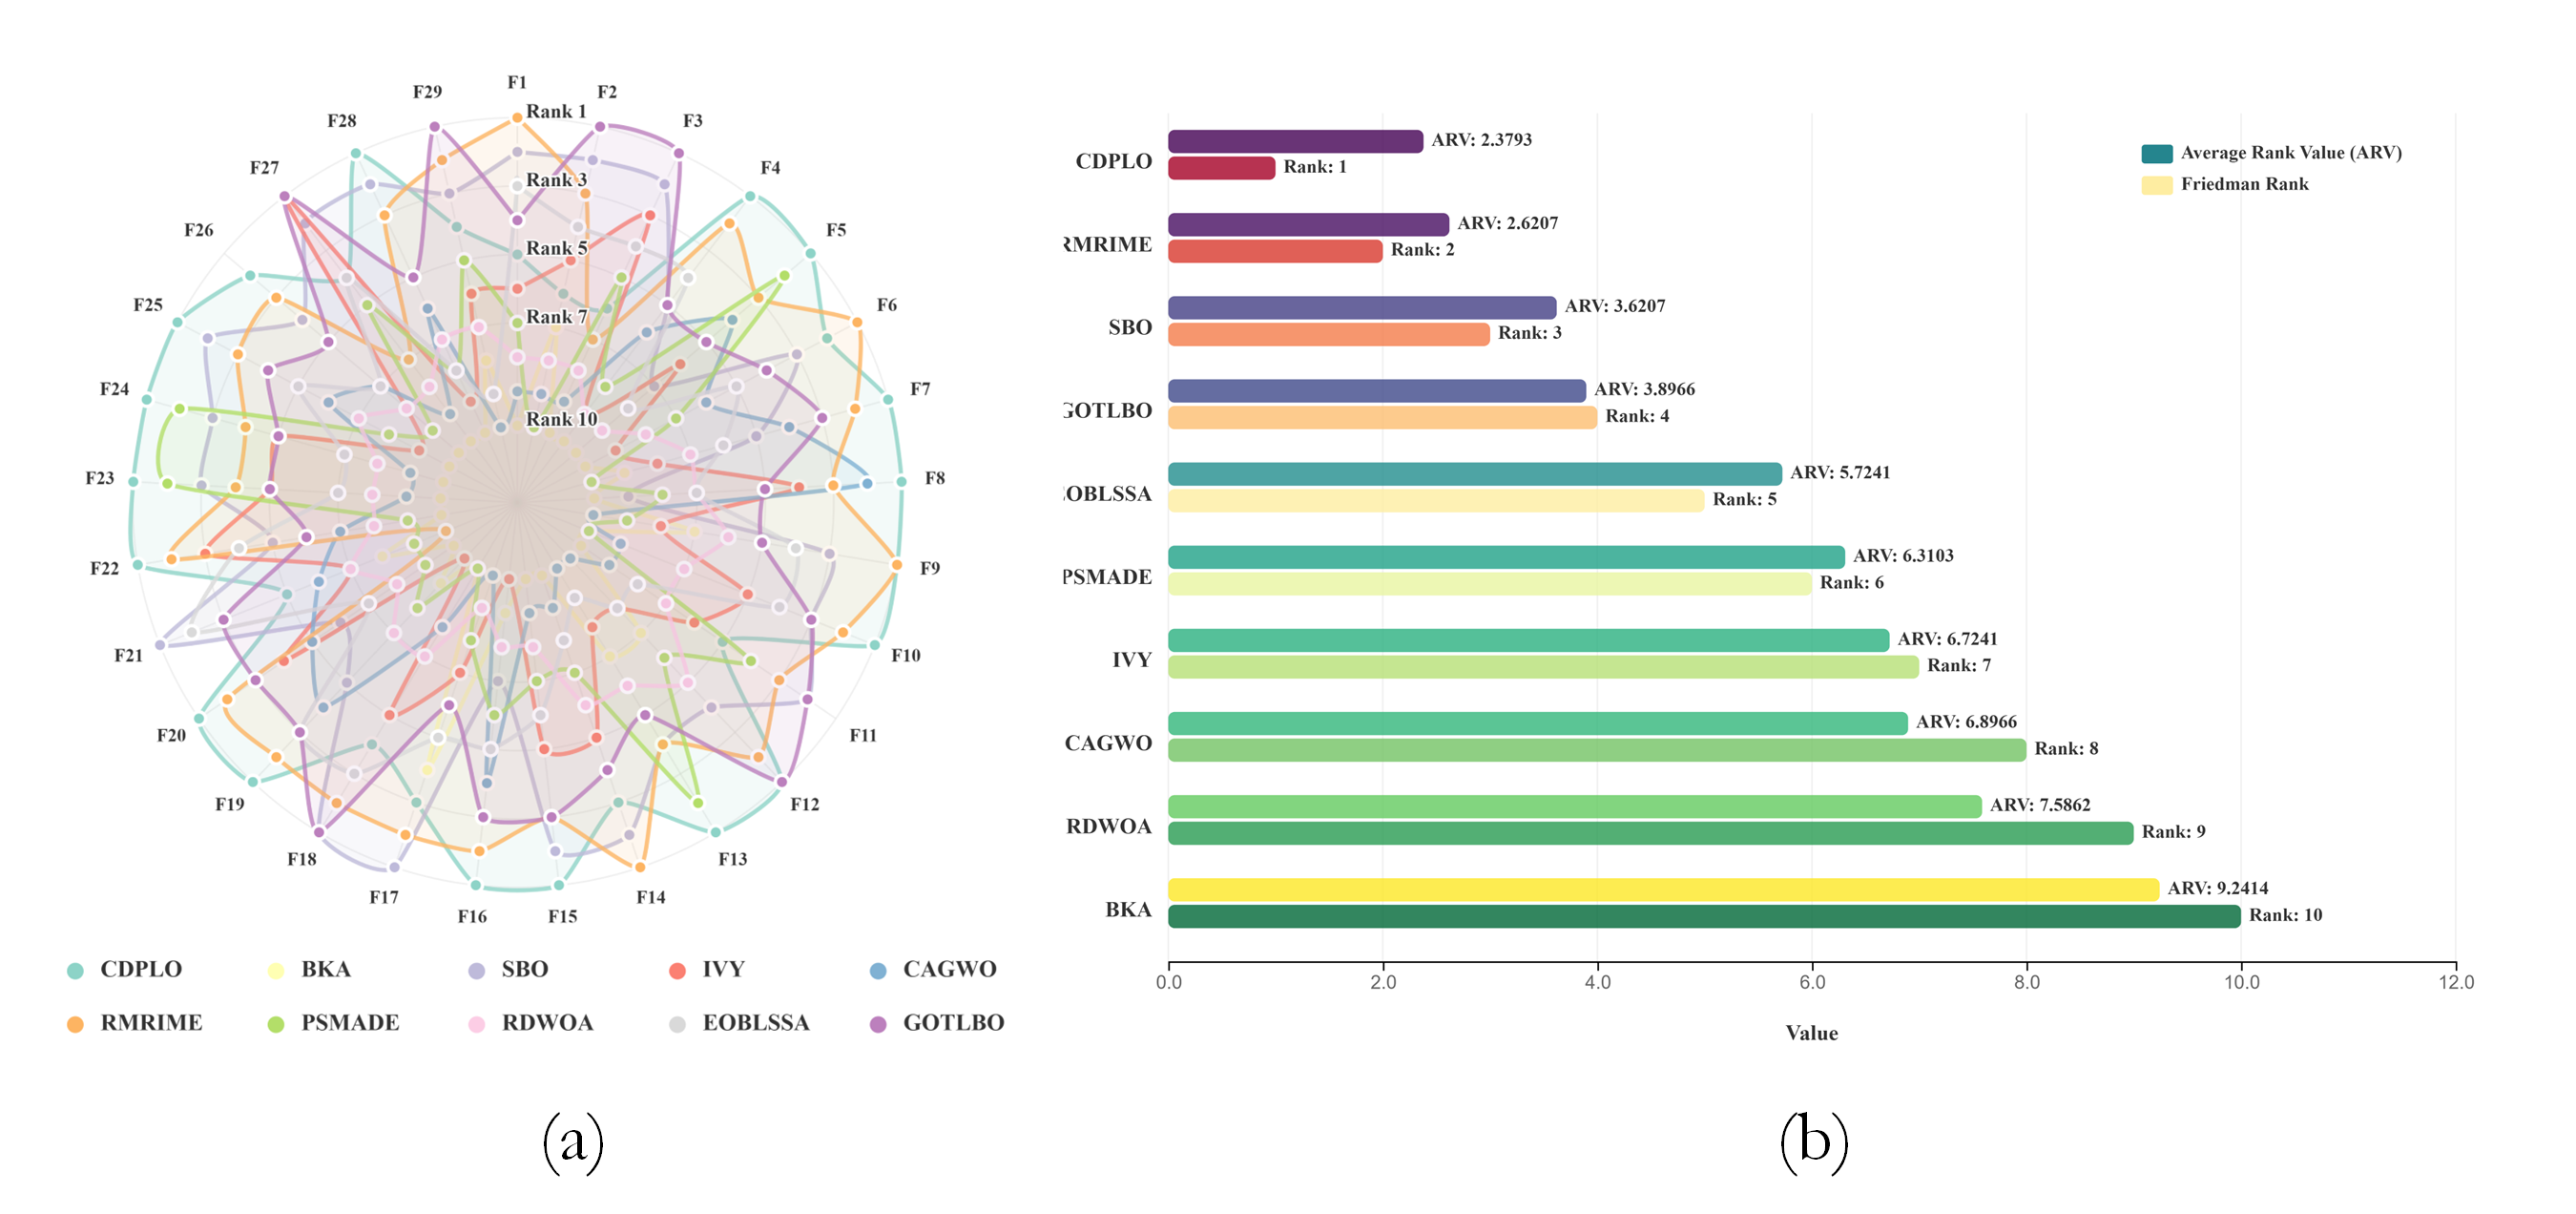
\includegraphics[width=\linewidth]{Cmp-FR}
\label{fig: Cmp-FR}
\end{figure}

\begin{table}
\centering
\begin{tabular}{@{} lcccccccccccccccc @{}}
\toprule
           & F1                 &                    & F2                 &                    & F3                 &                    & F4                 &                    & F5                 &                    & F6                   &                     & F7                 &                    & F8                 &                    \\ \midrule
Algorithms & Avg                & Std                & Avg                & Std                & Avg                & Std                & Avg                & Std                & Avg                & Std                & Avg                  & Std                 & Avg                & Std                & Avg                & Std                \\
CDPLO      & 5.842E+03          & 3.057E+03          & \textbf{1.022E+04} & 3.529E+03          & 4.948E+02          & 1.071E+01          & \textbf{5.441E+02} & 1.042E+01          & \textbf{6.005E+02} & \textbf{2.867E-01} & \textbf{8.048E+02}   & 1.364E+01           & 8.470E+02          & \textbf{6.478E+00} & \textbf{9.000E+02} & \textbf{4.418E-04} \\
CPLO       & 1.204E+04          & \textbf{2.374E+03} & 2.539E+04          & 5.531E+03          & 4.817E+02          & \textbf{8.858E+00} & 5.469E+02          & \textbf{7.580E+00} & 6.106E+02          & 2.153E+00          & 8.159E+02            & 1.591E+01           & 8.595E+02          & 8.397E+00          & 1.161E+03          & 9.314E+01          \\
DPLO       & \textbf{4.891E+03} & 2.924E+03          & 1.122E+04          & \textbf{3.506E+03} & 4.932E+02          & 9.055E+00          & 5.442E+02          & 9.469E+00          & 6.006E+02          & 3.426E-01          & 8.050E+02            & \textbf{1.033E+01}  & \textbf{8.447E+02} & 6.670E+00          & 9.000E+02          & 5.861E-04          \\
PLO        & 1.152E+04          & 2.482E+03          & 2.659E+04          & 5.377E+03          & \textbf{4.745E+02} & 1.412E+01          & 5.509E+02          & 7.811E+00          & 6.119E+02          & 2.170E+00          & 8.208E+02            & 1.762E+01           & 8.618E+02          & 1.353E+01          & 1.219E+03          & 1.261E+02          \\
           & F9                 &                    & F10                &                    & F11                &                    & F12                &                    & F13                &                    & F14                  &                     & F15                &                    & F16                &                    \\
Algorithms & Avg                & Std                & Avg                & Std                & Avg                & Std                & Avg                & Std                & Avg                & Std                & Avg                  & Std                 & Avg                & Std                & Avg                & Std                \\
CDPLO      & 4.125E+03          & \textbf{2.812E+02} & \textbf{1.145E+03} & 2.036E+01          & 5.615E+05          & 3.423E+05          & 1.753E+04          & 1.504E+04          & \textbf{1.852E+03} & \textbf{4.633E+02} & 4.904E+03            & 5.440E+03           & \textbf{1.859E+03} & 1.642E+02          & \textbf{1.775E+03} & 2.867E+01          \\
CPLO       & 3.304E+03          & 3.061E+02          & 1.158E+03          & \textbf{1.282E+01} & \textbf{4.193E+05} & 3.288E+05          & \textbf{1.364E+04} & 6.008E+03          & 7.576E+03          & 3.712E+03          & \textbf{3.811E+03}   & \textbf{7.657E+02}  & 1.923E+03          & \textbf{1.156E+02} & 1.795E+03          & \textbf{2.019E+01} \\
DPLO       & 4.198E+03          & 2.977E+02          & 1.148E+03          & 2.439E+01          & 6.724E+05          & 4.806E+05          & 2.063E+04          & 1.479E+04          & 2.531E+03          & 1.983E+03          & 4.807E+03            & 4.754E+03           & 1.895E+03          & 1.217E+02          & 1.783E+03          & 3.904E+01          \\
PLO        & \textbf{3.277E+03} & 3.238E+02          & 1.158E+03          & 1.628E+01          & 4.269E+05          & \textbf{2.217E+05} & 1.468E+04          & \textbf{3.776E+03} & 1.011E+04          & 4.829E+03          & 4.684E+03            & 1.397E+03           & 1.975E+03          & 1.225E+02          & 1.829E+03          & 4.650E+01          \\
           & F17                &                    & F18                &                    & F19                &                    & F20                &                    & F21                &                    & F22                  &                     & F23                &                    & F24                &                    \\
Algorithms & Avg                & Std                & Avg                & Std                & Avg                & Std                & Avg                & Std                & Avg                & Std                & Avg                  & Std                 & Avg                & Std                & Avg                & Std                \\
CDPLO      & 5.787E+04          & 3.512E+04          & 5.940E+03          & 5.884E+03          & \textbf{2.088E+03} & \textbf{5.257E+01} & \textbf{2.342E+03} & 9.317E+00          & 3.076E+03          & 1.434E+03          & 2.693E+03            & 1.146E+01           & 2.861E+03          & 7.326E+00          & 2.887E+03          & 4.184E-01          \\
CPLO       & 1.208E+05          & 6.141E+04          & 3.179E+03          & \textbf{7.899E+02} & 2.169E+03          & 5.910E+01          & 2.346E+03          & 2.516E+01          & \textbf{2.311E+03} & \textbf{4.373E+00} & 2.698E+03            & 7.392E+00           & 2.866E+03          & \textbf{6.529E+00} & 2.885E+03          & 1.415E+00          \\
DPLO       & \textbf{5.449E+04} & \textbf{3.183E+04} & 6.544E+03          & 6.183E+03          & 2.114E+03          & 5.853E+01          & 2.342E+03          & 9.737E+00          & 3.461E+03          & 1.572E+03          & \textbf{2.692E+03}   & 8.987E+00           & \textbf{2.859E+03} & 9.045E+00          & 2.887E+03          & \textbf{3.400E-01} \\
PLO        & 1.169E+05          & 4.591E+04          & \textbf{3.110E+03} & 8.667E+02          & 2.168E+03          & 5.400E+01          & 2.353E+03          & \textbf{8.224E+00} & 2.641E+03          & 8.616E+02          & 2.701E+03            & \textbf{6.094E+00}  & 2.869E+03          & 8.906E+00          & \textbf{2.885E+03} & 1.577E+00          \\
           & F25                &                    & F26                &                    & F27                &                    & F28                &                    & F29                &                    & \multicolumn{2}{c}{Statistical comparison} &                    &                    &                    &                    \\
Algorithms & Avg                & Std                & Avg                & Std                & Avg                & Std                & Avg                & Std                & Avg                & Std                & WSRT                 & FR                  &                    &                    &                    &                    \\
CDPLO      & 3.968E+03          & \textbf{1.126E+02} & 3.202E+03          & 5.059E+00          & 3.218E+03          & 1.478E+01          & \textbf{3.406E+03} & 3.801E+01          & 1.148E+04          & \textbf{2.484E+03} & \textbf{2.0345}      & \textbf{1}          &                    &                    &                    &                    \\
CPLO       & 3.950E+03          & 4.269E+02          & 3.203E+03          & \textbf{3.668E+00} & \textbf{3.214E+03} & \textbf{4.843E+00} & 3.466E+03          & 5.797E+01          & 1.885E+04          & 5.045E+03          & 2.6552               & 3                   &                    &                    &                    &                    \\
DPLO       & 3.997E+03          & 1.297E+02          & \textbf{3.202E+03} & 4.429E+00          & 3.222E+03          & 1.997E+01          & 3.406E+03          & \textbf{3.078E+01} & \textbf{1.036E+04} & 4.291E+03          & 2.3448               & 2                   &                    &                    &                    &                    \\
PLO        & \textbf{3.811E+03} & 5.609E+02          & 3.202E+03          & 4.154E+00          & 3.214E+03          & 5.381E+00          & 3.441E+03          & 4.995E+01          & 2.039E+04          & 5.225E+03          & 2.9655               & 4                   &                    &                    &                    &                   \\ \bottomrule
\end{tabular}
\end{table}

\bibliography{CDPLO}

\end{document}
